\documentclass[a4paper,titlepage,11pt,twosides,floatssmall]{mwrep}
\usepackage[left=2.5cm,right=2.5cm,top=2.5cm,bottom=2.5cm]{geometry}
\usepackage[OT1]{fontenc}
\usepackage[utf8]{inputenc}
\usepackage{polski}
\usepackage{amsmath}
\usepackage{amsfonts}
\usepackage{amssymb}
\usepackage{graphicx}
\usepackage{url}
\usepackage{tikz}
\usetikzlibrary{arrows,calc,decorations.markings,math,arrows.meta}
\usepackage{rotating}
\usepackage[percent]{overpic}

\usepackage{xcolor}
\usepackage{pgfplots}
\usetikzlibrary{pgfplots.groupplots}
\usepackage{listings}
\usepackage{matlab-prettifier}
\usepackage{enumitem,amssymb}
\definecolor{szary}{rgb}{0.95,0.95,0.95}
\usepackage{siunitx}
\sisetup{detect-weight,exponent-product=\cdot,output-decimal-marker={,},per-mode=symbol,binary-units=true,range-phrase={-},range-units=single}
\SendSettingsToPgf
%konfiguracje pakietu listings
\lstset{
	numbers=left,
	stepnumber=1,
	firstnumber=1,
	numberfirstline=true,
	backgroundcolor=\color{szary},
	frame=single,
	breaklines=true,
}
\lstdefinestyle{customlatex}{
	basicstyle=\footnotesize\ttfamily,
	%basicstyle=\small\ttfamily,
}
\lstdefinestyle{customc}{
	breaklines=true,
	frame=tb,
	language=C,
	xleftmargin=0pt,
	showstringspaces=false,
	basicstyle=\small\ttfamily,
	keywordstyle=\bfseries\color{green!40!black},
	commentstyle=\itshape\color{purple!40!black},
	identifierstyle=\color{blue},
	stringstyle=\color{orange},
}
\lstdefinestyle{custommatlab}{
	captionpos=t,
	breaklines=true,
	frame=tb,
	xleftmargin=0pt,
	language=matlab,
	showstringspaces=false,
	%basicstyle=\footnotesize\ttfamily,
	basicstyle=\scriptsize\ttfamily,
	keywordstyle=\bfseries\color{green!40!black},
	commentstyle=\itshape\color{purple!40!black},
	identifierstyle=\color{blue},
	stringstyle=\color{orange},
}

%wymiar tekstu (bez żywej paginy)
\textwidth 160mm \textheight 247mm

%ustawienia pakietu pgfplots
\pgfplotsset{
tick label style={font=\scriptsize},
label style={font=\small},
legend style={font=\small},
title style={font=\small}
}

\def\figurename{Rys.}
\def\tablename{Tab.}

%konfiguracja liczby pływających elementów
\setcounter{topnumber}{0}%2
\setcounter{bottomnumber}{3}%1
\setcounter{totalnumber}{5}%3
\renewcommand{\textfraction}{0.01}%0.2
\renewcommand{\topfraction}{0.95}%0.7
\renewcommand{\bottomfraction}{0.95}%0.3
\renewcommand{\floatpagefraction}{0.35}%0.5

\begin{document}
\frenchspacing
\pagestyle{uheadings}

%strona tytułowa
\title{\bf Sprawozdanie z projektu i ćwiczenia laboratoryjnego nr 1, zadanie nr 1\vskip 0.1cm}
\author{Imię i Nazwisko, Imię i Nazwisko, Imię i Nazwisko}
\date{2017}

\makeatletter
\renewcommand{\maketitle}{\begin{titlepage}
\begin{center}{\LARGE {\bf
Wydział Elektroniki i Technik Informacyjnych}}\\
\vspace{0.4cm}
{\LARGE {\bf Politechnika Warszawska}}\\
\vspace{0.3cm}
\end{center}
\vspace{5cm}
\begin{center}
{\bf \LARGE Projektowanie układów sterowania\\ (projekt grupowy) \vskip 0.1cm}
\end{center}
\vspace{1cm}
\begin{center}
{\bf \LARGE \@title}
\end{center}
\vspace{2cm}
\begin{center}
{\bf \Large \@author \par}
\end{center}
\vspace*{\stretch{6}}
\begin{center}
\bf{\large{Warszawa, \@date\vskip 0.1cm}}
\end{center}
\end{titlepage}
}
\makeatother

\maketitle

\tableofcontents
\chapter{Wstęp}
\section{Cel projektu}
Celem projektu było zbadanie właściwości danego obiektu oraz próba regulacji z wykorzystaniem dyskretnych algorytmów PID oraz DMC w wersji analitycznej. Częścią zadania było również uwzględnienie ograniczeń sterowania narzuconych w treści projektu.
\section{Opis algorytmów}
\subsection{PID}
W zadaniu projektowym wykorzystany został regulator PID. Algorytm ten, na podstawie obliczonej wartości uchybu oraz dobranych nastaw, wyznacza wartość sterowania dla chwili k. Elementami struktury algorytmu są następujące stałe:
\begin{itemize}
	\item $K$ - stała proporcjonalna
	\item $T_i$ - stała całkowania
	\item $T_d$ - stała różniczkowania
	\item $T$ - czas próbkowania
\end{itemize}

Dobranie nastaw algorytmu oznacza znalezienie możliwie optymalnych nastaw zapewniających najlepszą jakość regulacji.
\par Po wyznaczeniu parametrów, należy obliczyć wpółczynniki prawa regulacji używając następujących wzorów:
\begin{equation}
    r_2 = \frac{KTd}{T}
\end{equation}
\begin{equation}
    r_1 = K(\frac{T}{2T_i}-\frac{2T_d}{T}-1)
\end{equation}
\begin{equation}
    r_0 = K(\frac{T}{2T_i}+\frac{T_d}{T}+1)
\end{equation}
Prawo regulacji rgulatora opisane jest równaniem:
\begin{equation}
    u(k) = r_2e(k-2)+r_1e(k-2)+r_0e(k) +u(k-1)
\end{equation}


\subsection{DMC}
Regulator DMC jest algorytmem predykcyjnym wyznaczjącym trajektorię sygnału wyjściowego oraz przyszłe przyrosty sterowań. DMC potrzebuje wcześniejszej informacji o obiekcie w postaci odpowiedzi skokowej. Parametrami algorytmu są:
\begin{itemize}
    \item D - horyzont dynamiki
    \item N - horyzont predykcji
    \item $N_u$ - horyzont sterownia
    \item $\lambda$ - kara za zmianę sterownia
\end{itemize}

Strojenie algorytmu polega na odpowiednim dobraniu parametrów tak, by zapewnić możliwie najlepszą jakość regulacji.

\par Aby otrzymać prawo regulacji, należy wyznaczyć szereg współczynników:
\newline Macierz dynamiczną oraz macierz K:
\begin{gather}
        M = \begin{bmatrix}
            s_1 & 0 & \cdots & 0\\
            s_2 & s_1 & \cdots & 0\\
            \vdots & \vdots & \ddots & \vdots \\
            s_N & s_{N-1} & \cdots & s_{N-N_u+1}
        \end{bmatrix} \\
         K = (M^T \Psi M + \Lambda)^{-1} M^T \Psi 
\end{gather}
\newline Macierz $M^P$ oraz wektor zmian sterowania $\Delta U^P$:
\begin{gather}
        M^P = \begin{bmatrix}
            s_2-s_1 & s_3-s_2 & \cdots & s_D-s_{D-1}\\
            s_3-s_1 & s_4-s_2 & \cdots & s_{D+1}-s_{D-1}\\
            \vdots & \vdots & \ddots & \vdots \\
            s_{N+1}-s_1 & s_{N+2}-s_2 & \cdots & s_{N+D-1}-s_{D-1}
        \end{bmatrix} \\
         \Delta U^P(k) = \begin{bmatrix}
            \Delta u(k-1)\\
            \Delta u(k-2)\\
            \vdots\\
            \Delta u(k-(D-1))
        \end{bmatrix}
\end{gather}

Na podstawie powyższych macierzy oraz wektorów, można obliczyć parametry reguatora:
\begin{gather}
        k_e = \sum^N_{i=1}K_{1,i}\\
	k_u = \overline{K}_1 M^P
\end{gather}

a następnie wyznaczyć sterowanie z następującego prawa regulacji:
\begin{gather}
	e(k) = y_{zad}(k) - y(k)\\
    	u(k|k) = u(k - 1) + k_e e(k) - k_u \Delta U^P(k)
\end{gather}

Ograniczenie wartości sygnału sterującego przez wartości maksymalną i minimalną wykonane jest w następujący sposób:
\begin{enumerate}
    \item jeżeli $u(k|k) < u_{min}$ wtedy $u(k|k) = u_{min}$
\item jeżeli jeżeli $u(k|k) > u_{max}$ wtedy $u(k|k) = u_{max}$
max
\item $u(k) = u(k|k)$
\end{enumerate}
\chapter{zad1}
\chapter{Badanie obiektu}
\section{Symulacja różnych odpowiedzi skokowych obiektu}

Poniżej zamieszczono kod programu przeprowadzającego symulację obiektu dla ustalonegych $u$  z przedziału $ \langle  U^{\textrm{min}}, U^{\textrm{max}}\rangle $ uzyskując różne odpowiedzi skokowe. 

\begin{lstlisting}[style=Matlab-editor, basicstyle=\tiny]
t_sim2 = 300;

%konstruowanie sygnalow sterujacych
step_tim = 0;

u_base = ones(1,step_tim)*u_pp;
u_step_temp = ones(1,t_sim2 - step_tim)*1.3;
u_step2_temp = ones(1,t_sim2 - step_tim);
u_step3_temp = ones(1,t_sim2 - step_tim)*1.6;

u_step = [u_base, u_step_temp];
u_step2 = [u_base, u_step2_temp];
u_step3 = [u_base, u_step3_temp];

y = ones(t_sim2, 1)*y_pp;
y2 = ones(t_sim2, 1)*y_pp;
y3 = ones(t_sim2, 1)*y_pp;

for k = 3:t_sim2
    if k-11 <= 0
        y(k) = symulacja_obiektu6Y(u_pp,u_pp,y(k-1),y(k-2));
        y2(k) = symulacja_obiektu6Y(u_pp,u_pp,y2(k-1),y2(k-2));
        y3(k) = symulacja_obiektu6Y(u_pp,u_pp,y3(k-1),y3(k-2));
    else
        y(k) = symulacja_obiektu6Y(u_step(k-10),u_step(k-11),y(k-1),y(k-2));
        y2(k) = symulacja_obiektu6Y(u_step2(k-10),u_step2(k-11),y2(k-1),y2(k-2));
        y3(k) = symulacja_obiektu6Y(u_step3(k-10),u_step3(k-11),y3(k-1),y3(k-2));      
    end
end
\end{lstlisting}

W wyniku przeprowadzenia symulacji, otrzymano następujące przebiegi:
\begin{figure}[h] 
\centering 
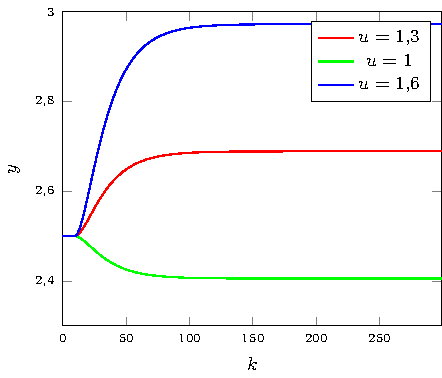
\includegraphics[scale=1.4]{wykresy/zad1_2/2_1.pdf} 
\caption{Odpowiedzi układu dla ustalonegych $u$  z przedziału $ \langle  U^{\textrm{min}}, U^{\textrm{max}}\rangle $ } 
\end{figure}

\par Na pierwszy rzut oka, obiekt wydaje się mieć liniową strukturę. Aby jednak to potwierdzić, należy wyznaczyć charakterystykę statyczną.


\section{Charakterystyka statyczna}
Aby wyznaczyć charakterystykę statyczną, stworzono symulację dla równiomiernie rozłożonych wartości sterowania z zakresu $ \langle  U^{\textrm{min}}, U^{\textrm{max}}\rangle $. Dla każdej z wartości sterowania wykonywano skok, a następnie czekano, aż wartość sygnału wyjściowego się ustabilizuje. Kod symulacji zamieszczony został poniżej:

\begin{lstlisting}[style=Matlab-editor]
t_sim = 400;
y_wyj = [];

for u = 0.6:0.01:1.6
    y = [0;0];
    for k=2:t_sim
        y_temp = symulacja_obiektu6Y(u,u,y(k),y(k-1));
        y = [y;y_temp];
    end
    y_wyj = [y_wyj; y(end)];
end
\end{lstlisting}

Poniżej zaprezentowany został wynik symulacji:
\begin{figure}[h] 
\centering 
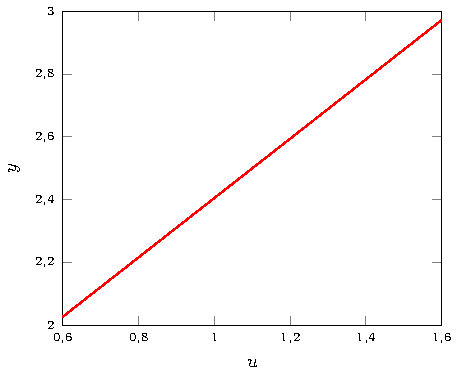
\includegraphics[scale=1.4]{wykresy/zad1_2/char_stat.pdf} 
\caption{Przybliżona charakterystyka statyczna układu} 
\end{figure}
Wyraźnie widać, że charakterystyka statyczna obiektu jest liniowa. Można zatem obliczyć wzmocnienie statyczne obiektu mając na uwadzę zależność:

\begin{equation}
K_{\textrm{stat}} = \frac{Y^{\textrm{max}} - Y^{\textrm{min}}}{U^{\textrm{max}} - U^{\textrm{min}}}
\end{equation}
Na podstawie powyższych rozważań obliczono $K_{\textrm{stat}} = \num{0.936}$




\chapter{Odpowiedź skokowa}
Odpowiedź skokowa to odpowiedź układu na wymuszenie w postaci skoku jednostkowego w chwili $k=0$. Z powodu ograniczeń sterowania obiektu, skok jednostkowy jest niemożliwy, dlatego należy przeskalować odpowiedź skokową w następujący sposób:
\begin{equation}
\triangle{S_i} = \frac{S_i^0-Y_{pp}}{\triangle{U}}\textrm{, dla } i=1,\ldots,N
\end{equation}
gdzie $N$ to wybrana długość odpowiedzi skokowej.
\begin{figure}[tb]
\centering
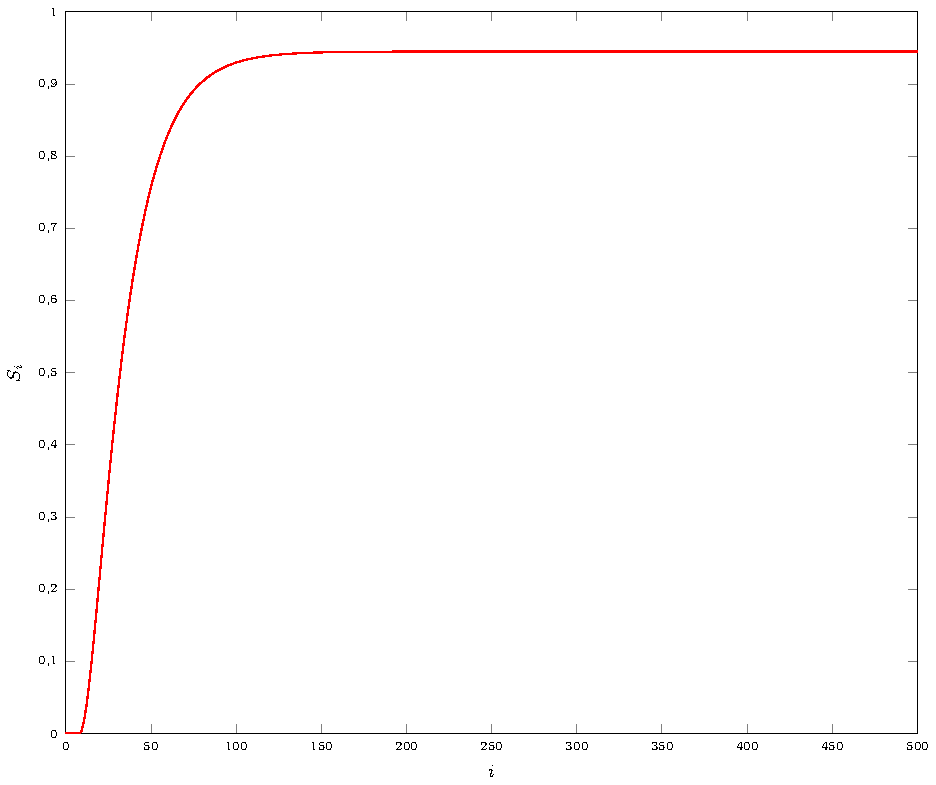
\includegraphics[scale=1]{wykresy/odp_skok}
\caption{Odpowiedź skokowa}
\label{odp_skok}
\end{figure}
Odpowiedź skokowa prezentowana na wykresie \ref{odp_skok} została otrzymana z przesklowania odpowiedzi obiektu po skoku z $u_{pp}=\num{1.1}$ do $u=\num{1.4}$.
\chapter{zad4}
\chapter{Dobranie nastaw regulatorów metodą eksperymentalną}
Zadanie 5 polegało na dobraniu nastaw regulatora PID i DMC metodą eksperymentalną w oparciu o przebiegi i wskaźnik jakości regulacji $E$:

\begin{equation}
    E = \sum_{k=1}^{k_{\mathrm{konc}}}(y^{\mathrm{zad}}(k)-y(k))^{2}
\end{equation}

dla zaproponowanej przez nas trajektorii zmian sygnału zadanego $y^{\mathrm{zad}}$ (Rys 6.1.).

\begin{figure}[tb] 
\centering 
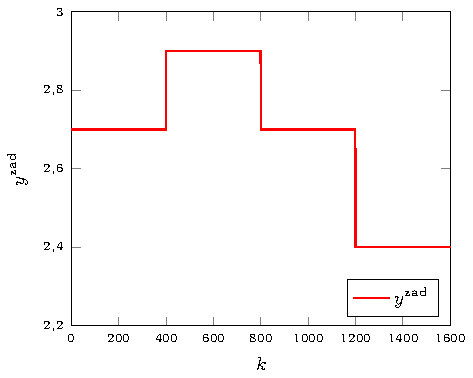
\includegraphics[scale=1]{rysunki/zapisz_pdf/y_zad.pdf} 
\caption{Trajektoria zmian sygnału $y^{\mathrm{zad}}$ na której przeprowadzimy symulacje} 
\label{r_pgfplots_trajektoria} 
\end{figure}

Ponieważ wskaźnik $E$ zliczany był już w poprzednim zadaniu, kod Matlabowy będzie tu taki sam jak w zadaniu 4.

\section{Eksperymentalne dobranie parametrów PID}
Do eksperymentalnego dobrania parametrów PID użyto nastepującej metody eksperymentalnej:
\begin{enumerate}
\item Zwiekszanie wpływu członu P przy wyłączonych członach I i D, aż dla pojedyńczego skoku wartości zadanej, wartość regulowana będzie wykonywała stałe, niegasnące oscylacje wokół wartości zadanej.
\item Dla wartości równej połowie uzyskanej w kroku pierwszym i wyłączonym członie D, dobranie wartości $T_{\mathrm{i}}$ dającej zadowalające wyniki.
\item Dla wartości $K$ i $T_{\mathrm{i}}$ dobranych w kroku drugim, dobranie wartości $T_{\mathrm{d}}$ dającej zadowalające wyniki.
\end{enumerate}


Stałe oscylacje obiektu osiągnięto dla $K_{\mathrm{kryt}}=\num{3.95}$ (Rys 6.2.).


\begin{figure}[tb] 
\centering 
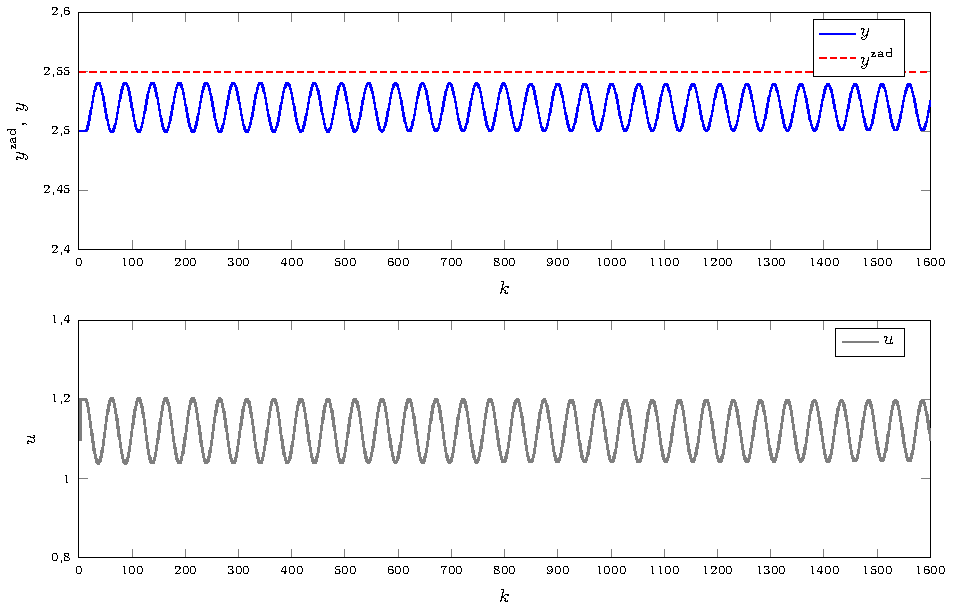
\includegraphics[scale=1]{rysunki/zapisz_pdf/oscylacje.pdf} 
\caption{Stałe (w pewnym przybliżeniu) oscylacje wartości wyjściowej $y$} 
\label{r_pgfplots_funkcje} 
\end{figure}


Warto zaznaczyć, że z powodu ograniczeń, każda wartość oscylacji powodująca ich rośnięcie doprowadzi w końcu do stałych oscylacji - należy więc być ostrożnym z dobieraniem parametru K, żeby parametr u nie został obcięty przez minimalizację, gdyż mogłoby to fałszywie sugerować stałość oscylacji.


Dla $K=\frac{1}{2}K_{\mathrm{kryt}}$ wyznaczonego z oscylacji otrzymujemy przebieg z Rys 6.3. 


\begin{figure}[tb] 
\centering 
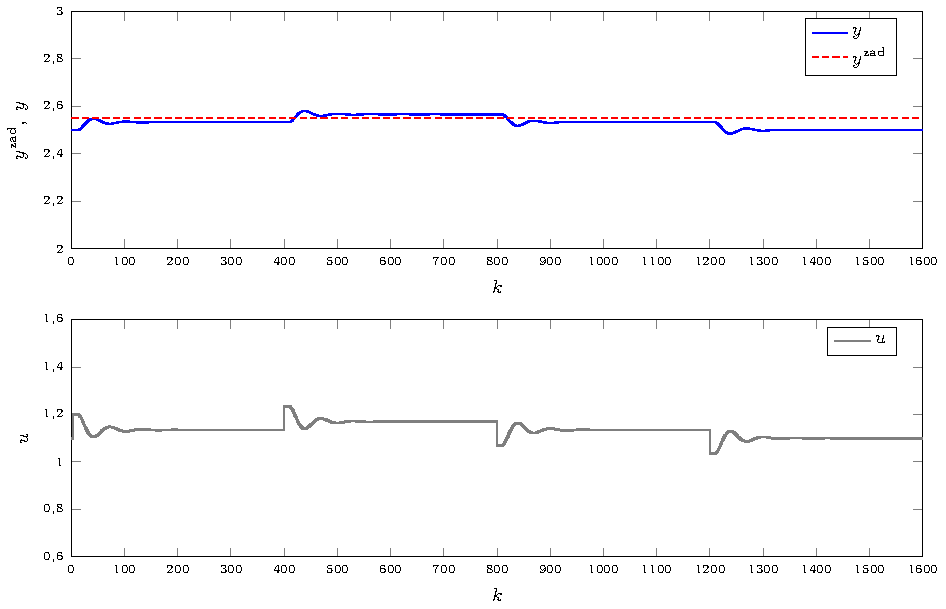
\includegraphics[scale=1]{rysunki/zapisz_pdf/PID_K=1.975_Ti=Inf_Td=0.00.pdf} 
\caption{Regulator PID dla $K=\num{1.975}$, $T_{\mathrm{i}}=inf$, $T_{\mathrm{d}}=0$} 
\label{r_pgfplots_PID_K=1.975_Ti=Inf_Td=0.00} 
\end{figure}

Uchyb ustalony jest zdecydowanie z wysoki, żeby uznać regulację za zadowalającą. Dobierzemy więc teraz parametr $T_{\mathrm{i}}$ włączając tym samym człon całkujący. Powinno pomóc to zredukować uchyb ustalony. Na rysunkach 6.4 - 6.12 przedstawiono regulację dla różnych, eksperymentalnie dobieranych wartości parametru $T_{\mathrm{i}}$.

\begin{figure}[tb] 
\centering 
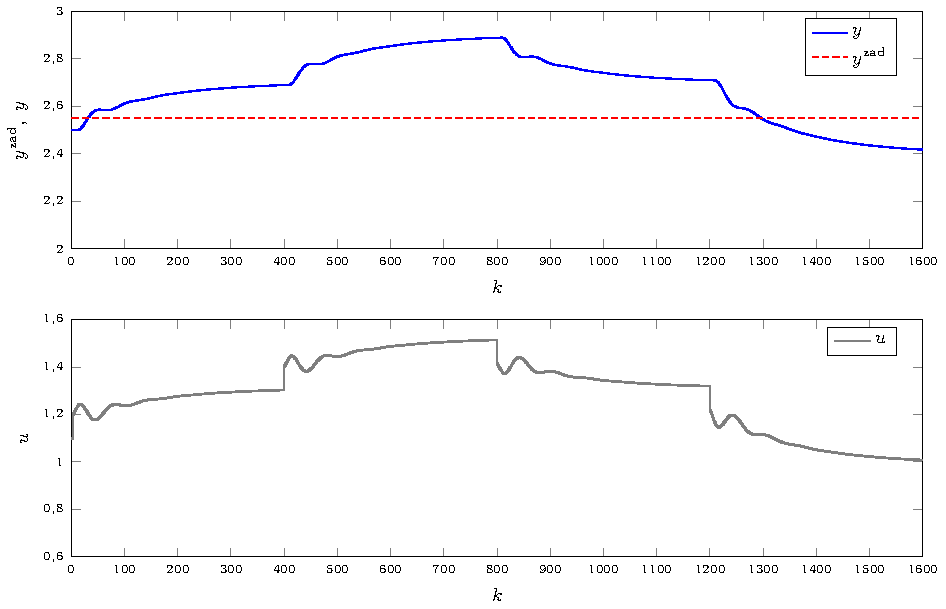
\includegraphics[scale=1]{rysunki/zapisz_pdf/PID_K=1.975_Ti=100.00_Td=0.00.pdf} 
\caption{Regulator PID dla $K=\num{1.975}$, $T_{\mathrm{i}}=100$, $T_{\mathrm{d}}=0$} 
\label{r_pgfplots_PID_K=1.975_Ti=100.00_Td=0.00} 
\end{figure}

\begin{figure}[tb] 
\centering 
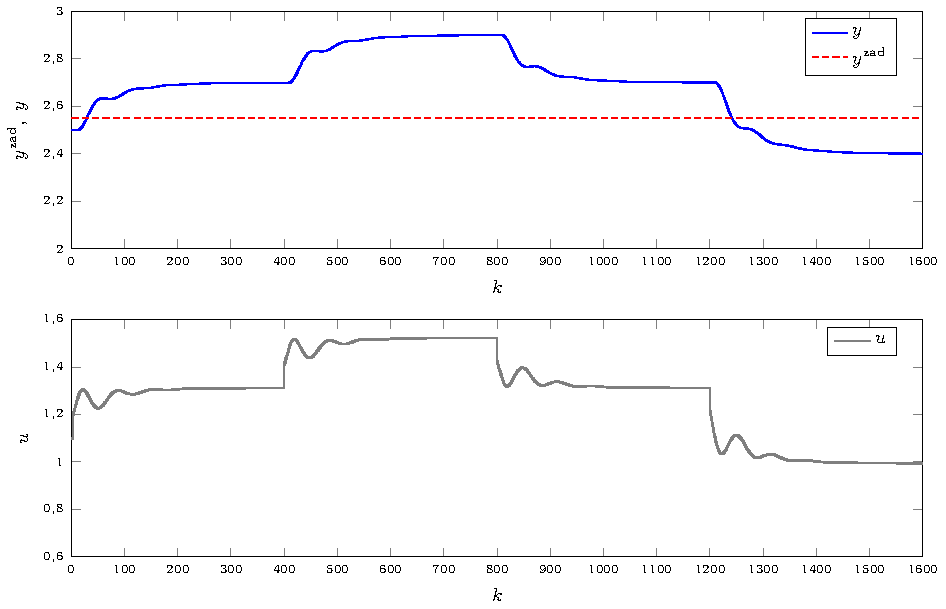
\includegraphics[scale=1]{rysunki/zapisz_pdf/PID_K=1.975_Ti=50.00_Td=0.00.pdf} 
\caption{Regulator PID dla $K=\num{1.975}$, $T_{\mathrm{i}}=50$, $T_{\mathrm{d}}=0$} 
\label{r_pgfplots_PID_K=1.975_Ti=50.00_Td=0.00} 
\end{figure}

\begin{figure}[tb] 
\centering 
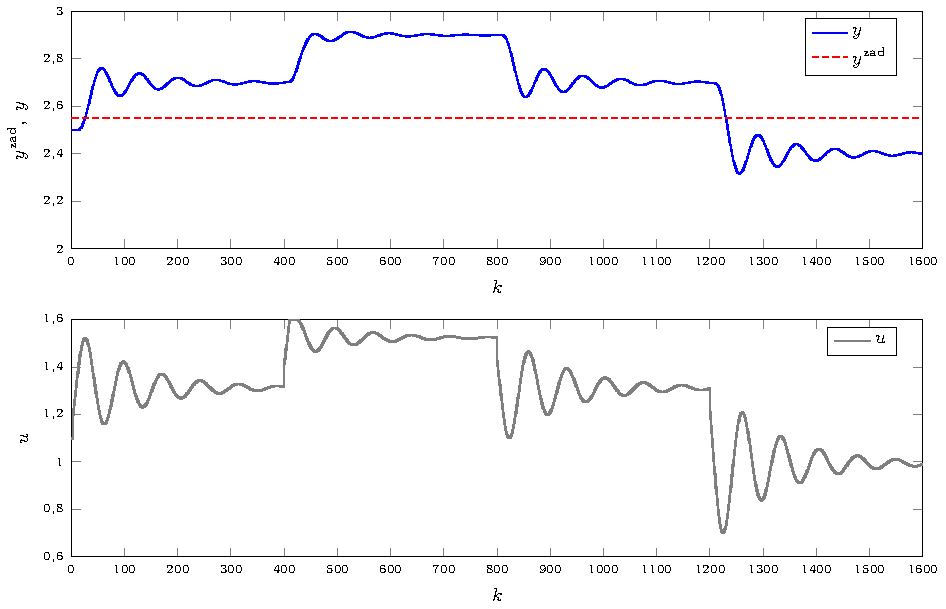
\includegraphics[scale=1]{rysunki/zapisz_pdf/PID_K=1.975_Ti=20.00_Td=0.00.pdf} 
\caption{Regulator PID dla $K=\num{1.975}$, $T_{\mathrm{i}}=20$, $T_{\mathrm{d}}=0$} 
\label{r_pgfplots_PID_K=1.975_Ti=20.00_Td=0.00} 
\end{figure}

\begin{figure}[tb] 
\centering 
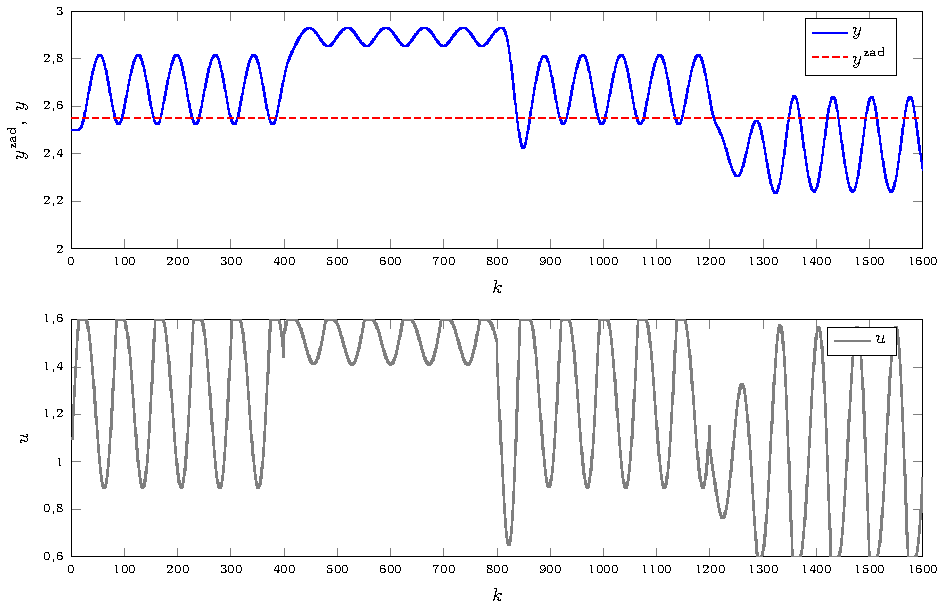
\includegraphics[scale=1]{rysunki/zapisz_pdf/PID_K=1.975_Ti=10.00_Td=0.00.pdf} 
\caption{Regulator PID dla $K=\num{1.975}$, $T_{\mathrm{i}}=10$, $T_{\mathrm{d}}=0$} 
\label{r_pgfplots_PID_K=1.975_Ti=10.00_Td=0.00} 
\end{figure}

\begin{figure}[tb] 
\centering 
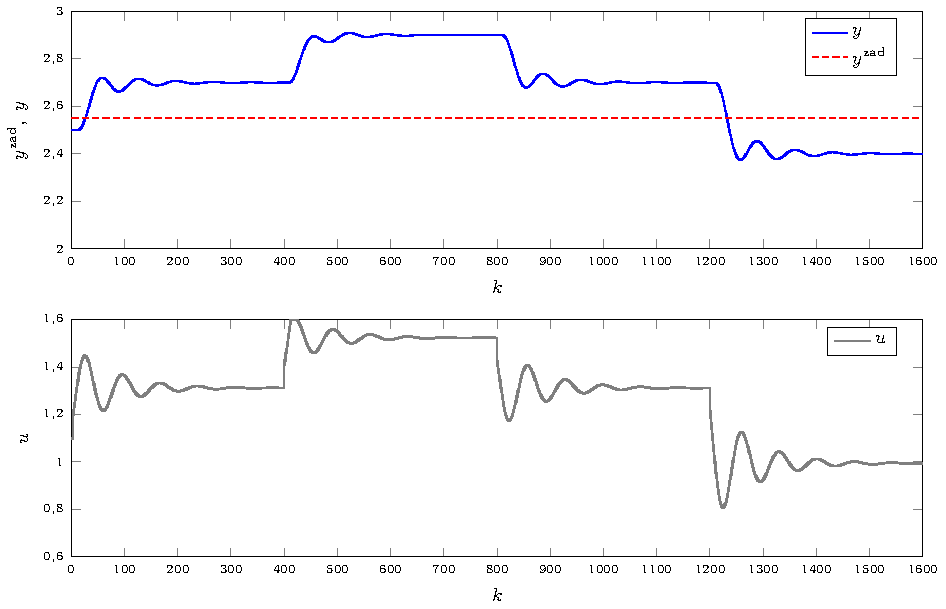
\includegraphics[scale=1]{rysunki/zapisz_pdf/PID_K=1.975_Ti=25.00_Td=0.00.pdf} 
\caption{Regulator PID dla $K=\num{1.975}$, $T_{\mathrm{i}}=25$, $T_{\mathrm{d}}=0$} 
\label{r_pgfplots_PID_K=1.975_Ti=25.00_Td=0.00} 
\end{figure}

\begin{figure}[tb] 
\centering 
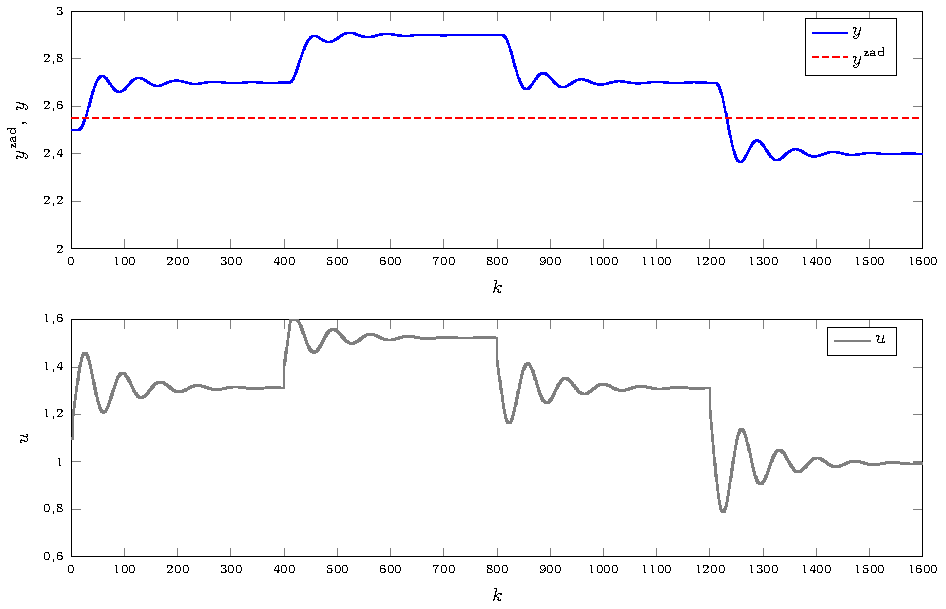
\includegraphics[scale=1]{rysunki/zapisz_pdf/PID_K=1.975_Ti=24.00_Td=0.00.pdf} 
\caption{Regulator PID dla $K=\num{1.975}$, $T_{\mathrm{i}}=24$, $T_{\mathrm{d}}=0$} 
\label{r_pgfplots_PID_K=1.975_Ti=24.00_Td=0.00} 
\end{figure}

\begin{figure}[tb] 
\centering 
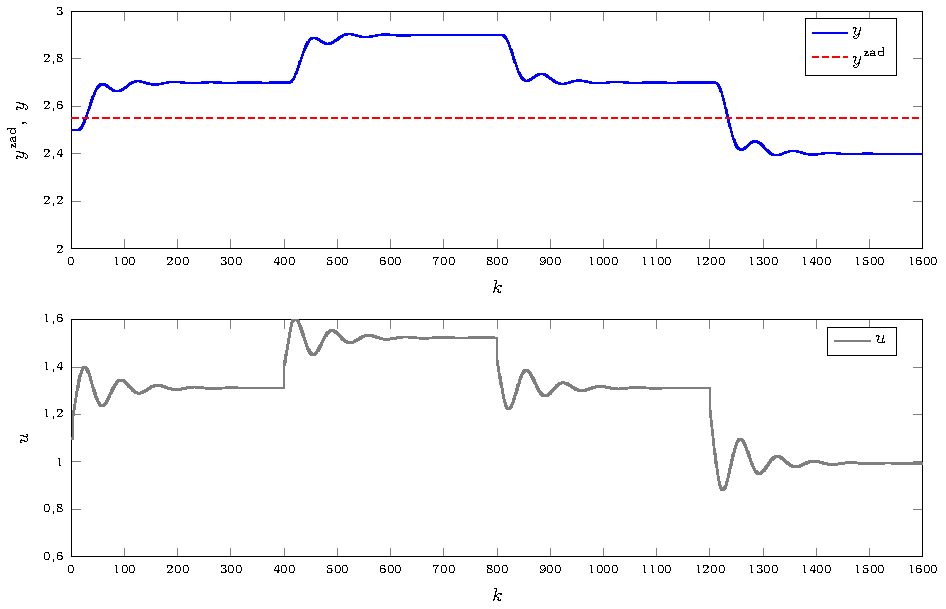
\includegraphics[scale=1]{rysunki/zapisz_pdf/PID_K=1.975_Ti=30.00_Td=0.00.pdf} 
\caption{Regulator PID dla $K=\num{1.975}$, $T_{\mathrm{i}}=30$, $T_{\mathrm{d}}=0$} 
\label{r_pgfplots_PID_K=1.975_Ti=30.00_Td=0.00} 
\end{figure}

\begin{figure}[tb] 
\centering 
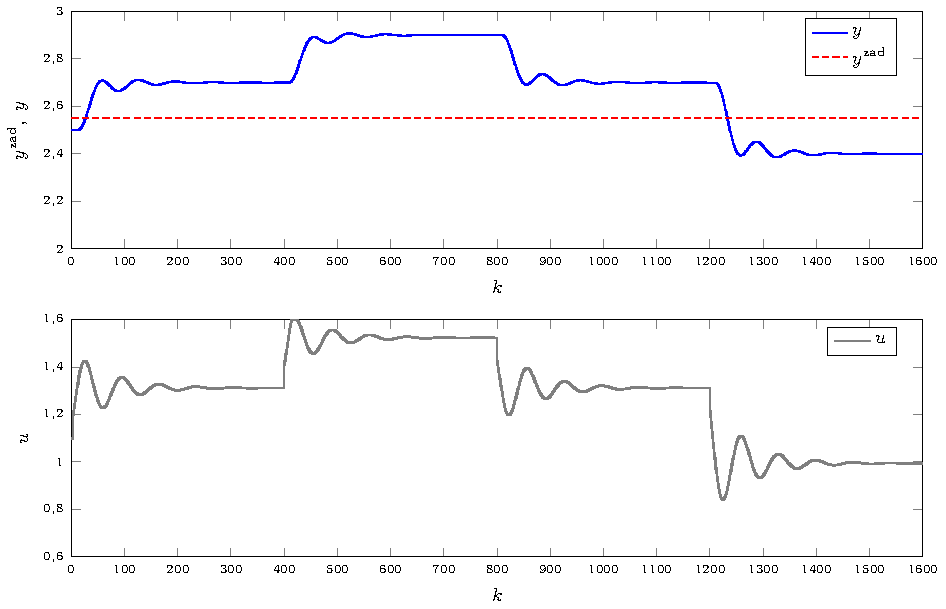
\includegraphics[scale=1]{rysunki/zapisz_pdf/PID_K=1.975_Ti=27.00_Td=0.00.pdf} 
\caption{Regulator PID dla $K=\num{1.975}$, $T_{\mathrm{i}}=27$, $T_{\mathrm{d}}=0$} 
\label{r_pgfplots_PID_K=1.975_Ti=27.00_Td=0.00} 
\end{figure}

\begin{figure}[tb] 
\centering 
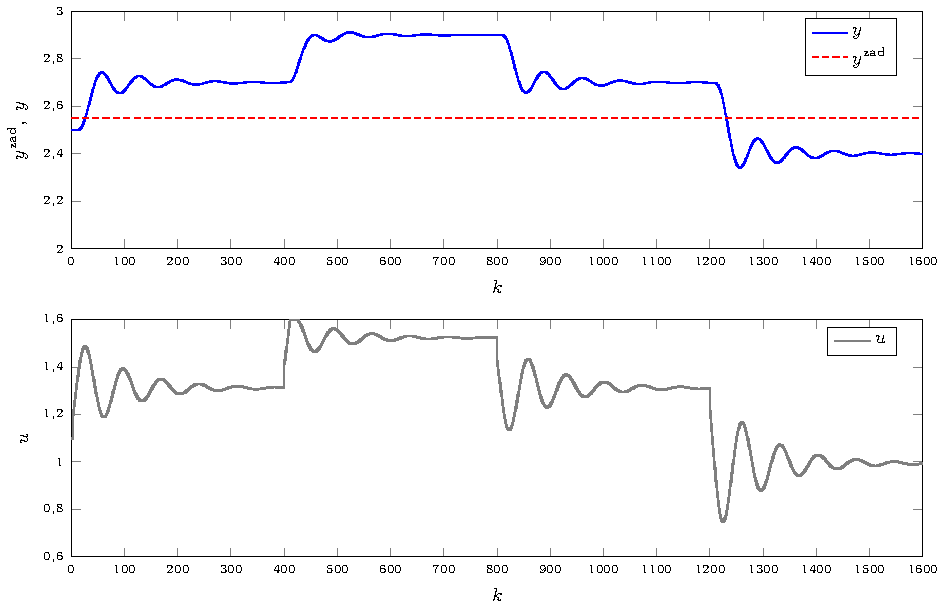
\includegraphics[scale=1]{rysunki/zapisz_pdf/PID_K=1.975_Ti=22.00_Td=0.00.pdf} 
\caption{Regulator PID dla $K=\num{1.975}$, $T_{\mathrm{i}}=22$, $T_{\mathrm{d}}=0$} 
\label{r_pgfplots_PID_K=1.975_Ti=22.00_Td=0.00} 
\end{figure}


\begin{table}
	[b] \caption{Porównanie wielkości błędu $E$ dla różnych wartości parametru $T_{\mathrm{i}}$ i dla parametru $K=\num{1.975}$}
	\label{t_T_i}
	\centering
	\sisetup{table-auto-round=true}
	\begin{small}
		\begin{tabular}{|c|c|}
			\hline
			$T_{\mathrm{i}}$	&	$E$	\\
			$inf$	&	$\num{71.3457}$		\\
			$100$ 	&	$\num{13.9366}$		\\
			$50$	&	$\num{7.8122}$		\\
			$30$	&	$\num{5.8606}$		\\
			$27$	&	$\num{5.6896}$		\\
			$25$	&	$\num{5.6210}$		\\
			$24$	&	$\num{5.6081}$		\\
			$22$	&	$\num{5.6506}$		\\
			$20$	&	$\num{5,8522}$		\\
			$10$	&	$\num{18.3320}$		\\
			\hline
			\end{tabular}
	\end{small}
\end{table}

Widzimiy, że najmniejszy błąd $E$ wystąpił dla $T_{/mathrm{i}}=24$ . Warto też zauważyć, że dla mniejszych wartości $T_{\mathrm{i}}$ zaczęły występować wolno gasnące oscylacje wartości wyjściowej. Jak widać jednak na Rys 6.9, oscylacje te są na tyle małe i gasną wystarczająco szybko, że można je tolerować. Następnym krokiem jest dobranie parametru $T_{\mathrm{d}}$. Dobierany był dla parametru $K=\num{1.975}$ i parametru $T_{\mathrm{i}}=24$.

\begin{figure}[tb] 
\centering 
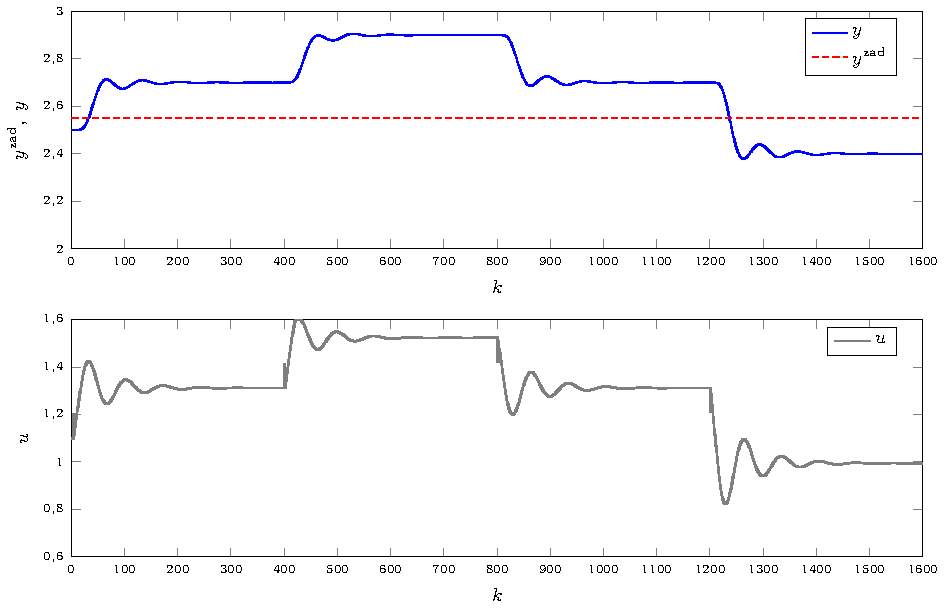
\includegraphics[scale=1]{rysunki/zapisz_pdf/PID_K=1.975_Ti=24.00_Td=1.00.pdf} 
\caption{Regulator PID dla $K=\num{1.975}$, $T_{\mathrm{i}}=24$, $T_{\mathrm{d}}=1$} 
\label{r_pgfplots_PID_K=1.975_Ti=24.00_Td=1.00} 
\end{figure}

\begin{figure}[tb] 
\centering 
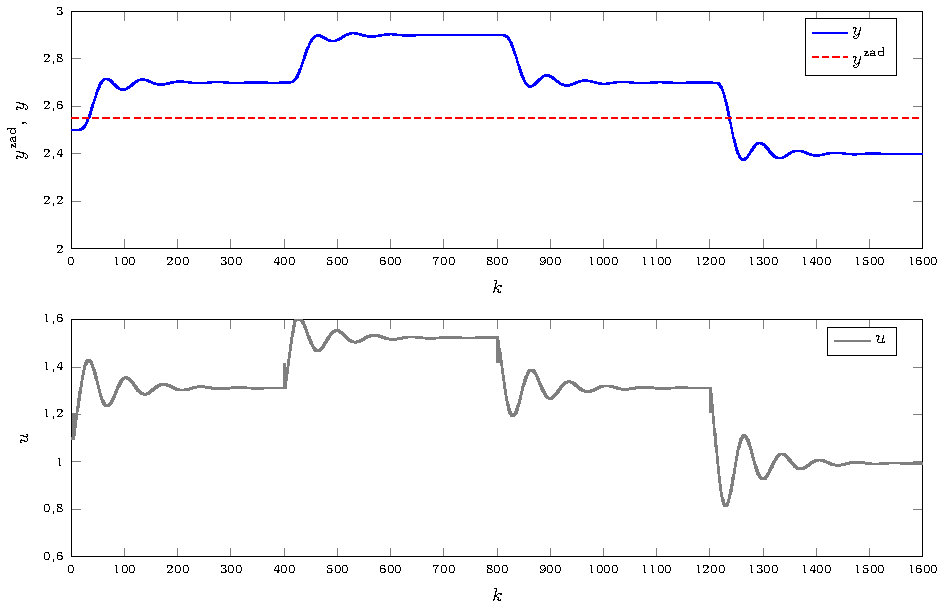
\includegraphics[scale=1]{rysunki/zapisz_pdf/PID_K=1.975_Ti=24.00_Td=0.50.pdf} 
\caption{Regulator PID dla $K=\num{1.975}$, $T_{\mathrm{i}}=24$, $T_{\mathrm{d}}=\num{0.5}$} 
\label{r_pgfplots_PID_K=1.975_Ti=24.00_Td=0.50} 
\end{figure}

\begin{figure}[tb] 
\centering 
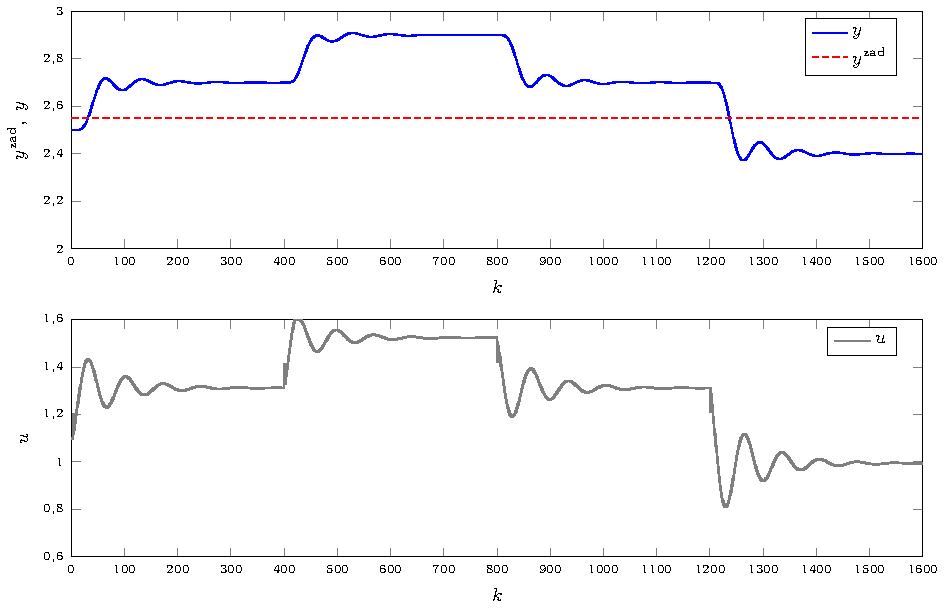
\includegraphics[scale=1]{rysunki/zapisz_pdf/PID_K=1.975_Ti=24.00_Td=0.25.pdf} 
\caption{Regulator PID dla $K=\num{1.975}$, $T_{\mathrm{i}}=24$, $T_{\mathrm{d}}=\num{0.25}$} 
\label{r_pgfplots_PID_K=1.975_Ti=24.00_Td=0.25} 
\end{figure}

\begin{figure}[tb] 
\centering 
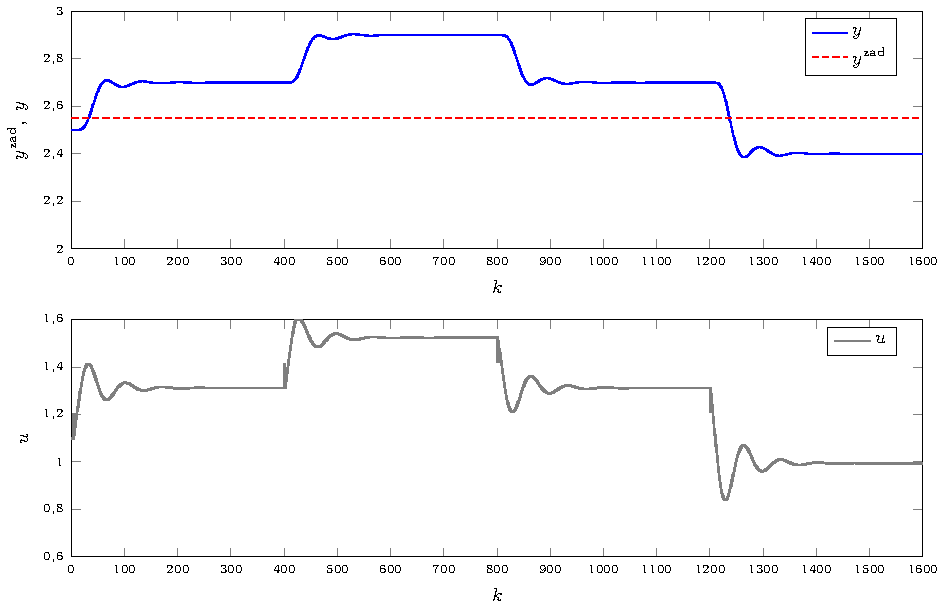
\includegraphics[scale=1]{rysunki/zapisz_pdf/PID_K=1.975_Ti=24.00_Td=2.00.pdf} 
\caption{Regulator PID dla $K=\num{1.975}$, $T_{\mathrm{i}}=24$, $T_{\mathrm{d}}=2$} 
\label{r_pgfplots_PID_K=1.975_Ti=24.00_Td=2.00} 
\end{figure}

\begin{figure}[tb] 
\centering 
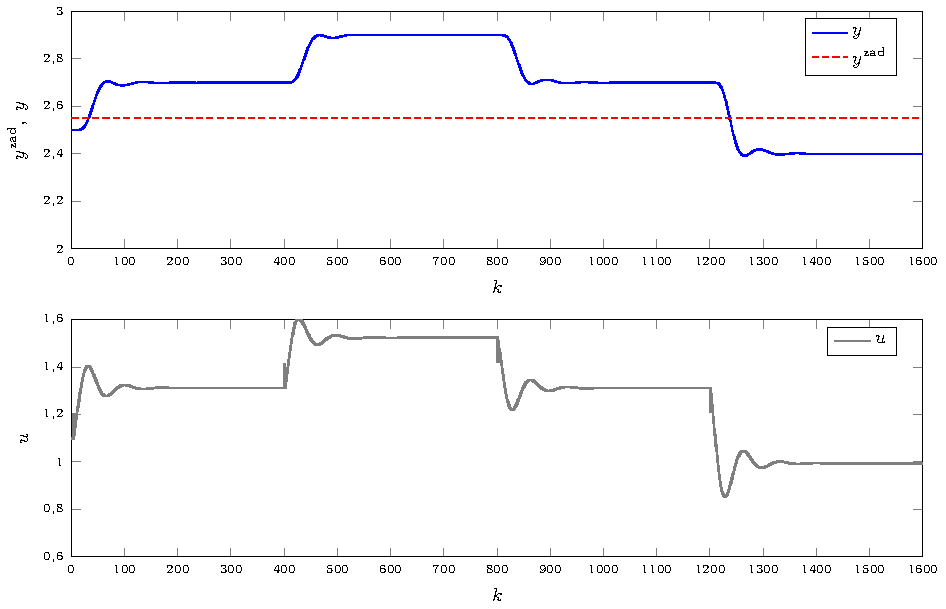
\includegraphics[scale=1]{rysunki/zapisz_pdf/PID_K=1.975_Ti=24.00_Td=3.00.pdf} 
\caption{Regulator PID dla $K=\num{1.975}$, $T_{\mathrm{i}}=24$, $T_{\mathrm{d}}=3$} 
\label{r_pgfplots_PID_K=1.975_Ti=24.00_Td=3.00} 
\end{figure}

\begin{figure}[tb] 
\centering 
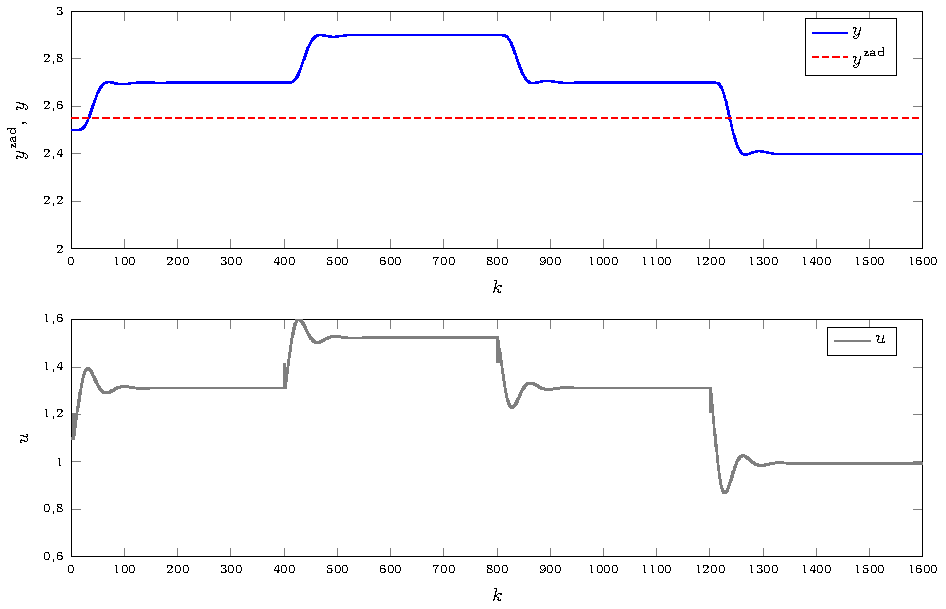
\includegraphics[scale=1]{rysunki/zapisz_pdf/PID_K=1.975_Ti=24.00_Td=4.00.pdf} 
\caption{Regulator PID dla $K=\num{1.975}$, $T_{\mathrm{i}}=24$, $T_{\mathrm{d}}=4$} 
\label{r_pgfplots_PID_K=1.975_Ti=24.00_Td=4.00} 
\end{figure}

\begin{table}
	[b] \caption{Porównanie wielkości błędu $E$ dla różnych wartości parametru $T_{\mathrm{d}}$ i dla parametru $K=1.975$ oraz parametru $T_{\mathrm{i}}=24$}
	\label{t_T_i}
	\centering
	\sisetup{table-auto-round=true}
	\begin{small}
		\begin{tabular}{|c|c|}
			\hline
			$T_{\mathrm{d}}$	&	$E$	\\
			$0$		&	$\num{5.6081}$		\\
			$\num{0.5}$ 	&	$\num{6.6090}$		\\
			$\num{0.25}	$ & $\num{6.4963}$ \\
			$1$ 	&	$\num{6.5853}$		\\
			$2$		&	$\num{6.5632}$	\\
			$3$		&	$\num{6.5644}$	\\
			$4$		&	$\num{6.5808}$	\\
			\hline
			\end{tabular}
	\end{small}
\end{table}

Jak widać z tabelki dodanie członu różniczkującego zwiększyło wartość błędu $E$. Na rysunkach widać jednak, że wystepujące wcześniej oscylacje znacznie zmniejszyły się dzięki działaniu członu, co jest pożądane, zwłaszcza dla obiektów rzeczywistych. Można dobrać różne wartości $T_{\mathrm{d}}$ w zależności od pożądanego tłumienia oscylacji, jako kompromis między tłumieniem a wskaźnikiem jakości $E$ wybrane zostało $T_{\mathrm{d}}=3$ (Rys 6.17). Ostateczne parametry PID otrzymane w wyniku eksperymentów to: $K=\num{1.975}$, $T_{\mathrm{i}}=24$, $T_{\mathrm{d}}=3$. Oczywiście nie są to pewnie idealne parametry regulatora.


\section{Eksperymentalne dobranie parametrów DMC}

Do eksperymentalnego dobrania parametrów DMC użyto nastepującej metody eksperymentalnej:
\begin{enumerate}
\item Przyjęcie maksymalnego możliwego parametry $D$, równego długości odpowiedzi skokowej aż do jej ustabilizowania, w naszym przypadku $D=200$. 
\item Dla maksymalnie dużego parametru $D$ stopniowe zmniejszanie parametrów $N$ i $N_{\mathrm{u}}$ ($N$ musi byc cały czas równe $N_{\mathrm{u}}$, aż osiągniemy zadowalające wyniki.
\item Dla tak dobranych parametrów $D$ i $N$ dobranie parametru $N_{\mathrm{u}}$ dającego zadowalające wyniki.
\end{enumerate}


Wyjściowy regulator DMC ($D=N=N_{\mathrm{u}}=200$) przeedstawiony jest na Rys 6.13. Po błędzie i ryunku widać, że już i taki regulator DMC sprawia się lepiej niż regulator PID. Ponieważ dla wartości $N\ge{50}$ regulator zachowywał się w przybliżeniu identycznie nie zamieszczone zostały wykresy dla nich.


\begin{figure}[tb] 
\centering 
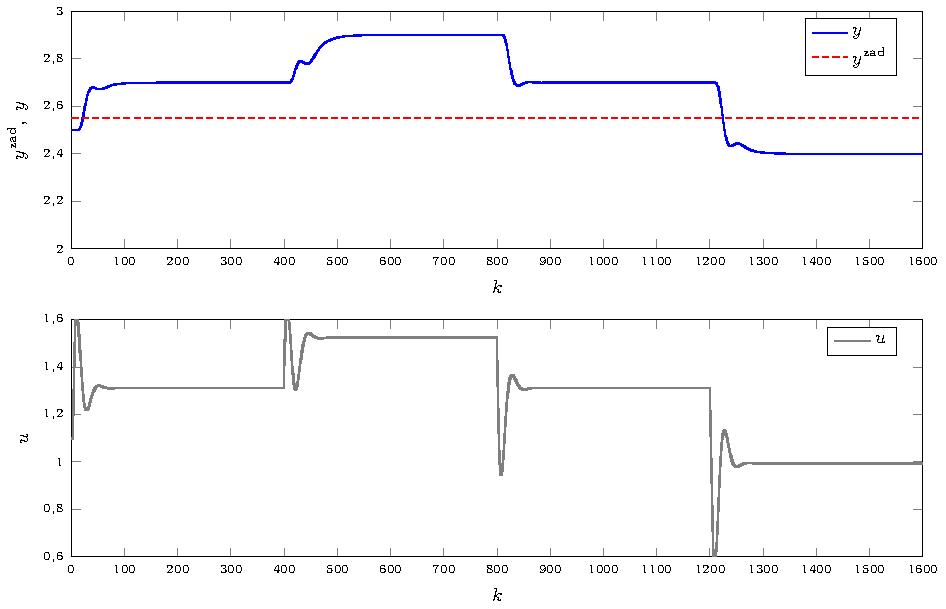
\includegraphics[scale=1]{rysunki/zapisz_pdf/DMC_D=200.000_N=200.00_Nu=200.00.pdf} 
\caption{Regulator DMC dla $D=200$, $N=200$, $N_{\mathrm{u}}=200$} 
\label{r_pgfplots_DMC_D=200.000_N=200.00_Nu=200.00} 
\end{figure}

\begin{figure}[tb] 
\centering 
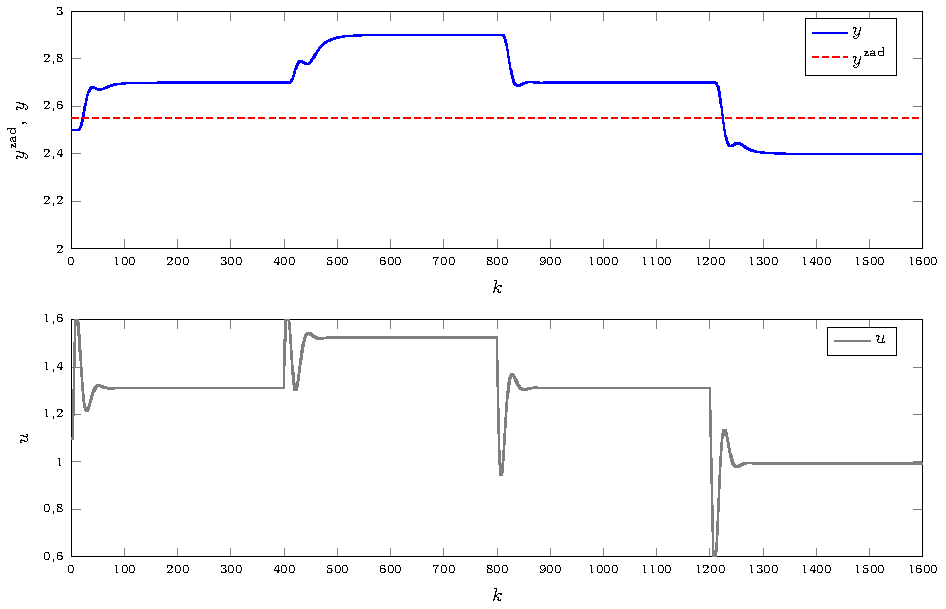
\includegraphics[scale=1]{rysunki/zapisz_pdf/DMC_D=200.000_N=40.00_Nu=40.00.pdf} 
\caption{Regulator DMC dla $D=200$, $N=40$, $N_{\mathrm{u}}=40$} 
\label{r_pgfplots_DMC_D=200.000_N=40.00_Nu=40.00} 
\end{figure}

\begin{figure}[tb] 
\centering 
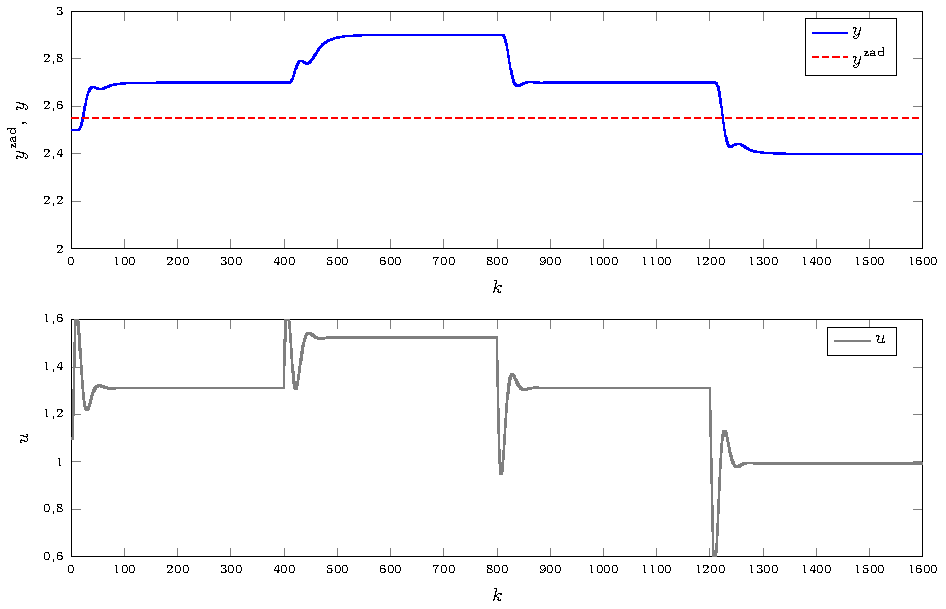
\includegraphics[scale=1]{rysunki/zapisz_pdf/DMC_D=200.000_N=30.00_Nu=30.00.pdf} 
\caption{Regulator DMC dla $D=200$, $N=30$, $N_{\mathrm{u}}=30$} 
\label{r_pgfplots_DMC_D=200.000_N=30.00_Nu=30.00} 
\end{figure}

\begin{figure}[tb] 
\centering 
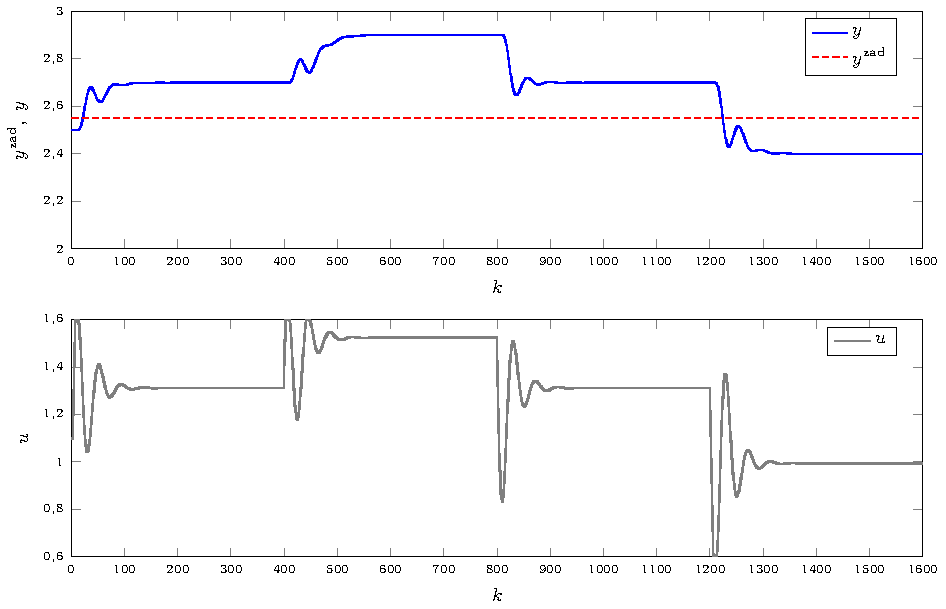
\includegraphics[scale=1]{rysunki/zapisz_pdf/DMC_D=200.000_N=20.00_Nu=20.00.pdf} 
\caption{Regulator DMC dla $D=200$, $N=20$, $N_{\mathrm{u}}=20$} 
\label{r_pgfplots_DMC_D=200.000_N=20.00_Nu=20.00} 
\end{figure}

\begin{figure}[tb] 
\centering 
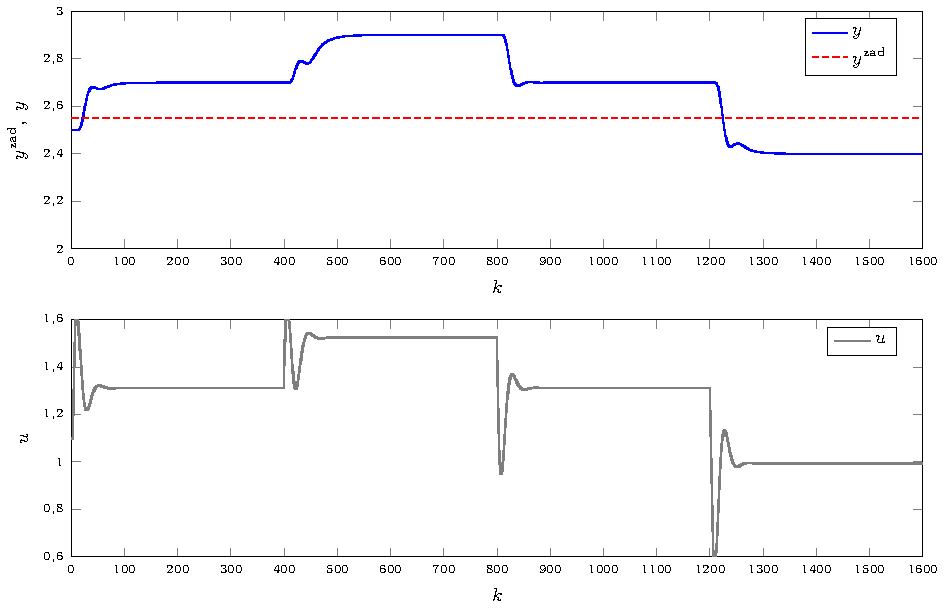
\includegraphics[scale=1]{rysunki/zapisz_pdf/DMC_D=200.000_N=35.00_Nu=35.00.pdf} 
\caption{Regulator DMC dla $D=200$, $N=35$, $N_{\mathrm{u}}=35$} 
\label{r_pgfplots_DMC_D=200.000_N=35.00_Nu=35.00} 
\end{figure}

\begin{figure}[tb] 
\centering 
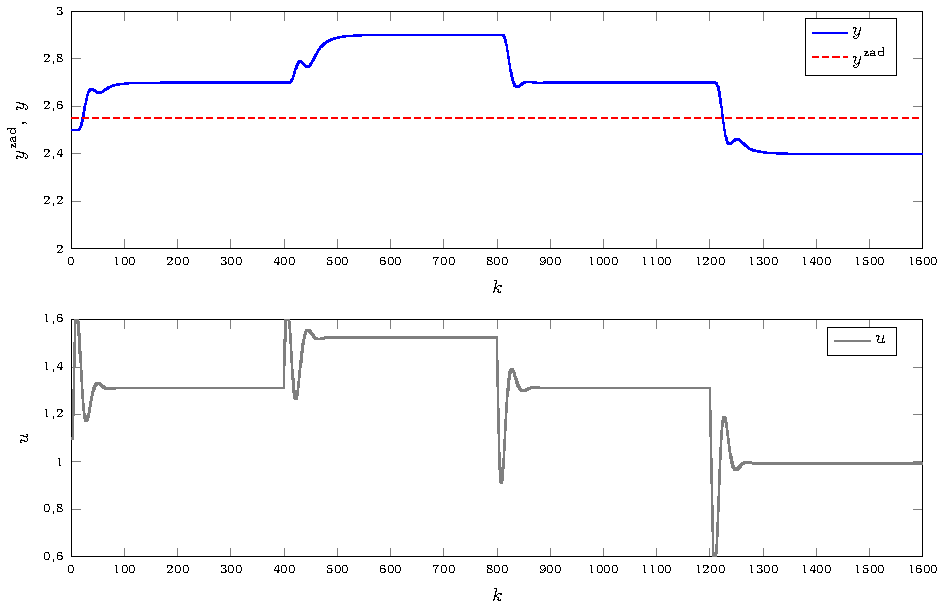
\includegraphics[scale=1]{rysunki/zapisz_pdf/DMC_D=200.000_N=25.00_Nu=25.00.pdf} 
\caption{Regulator DMC dla $D=200$, $N=25$, $N_{\mathrm{u}}=25$} 
\label{r_pgfplots_DMC_D=200.000_N=25.00_Nu=25.00} 
\end{figure}

\begin{figure}[tb] 
\centering 
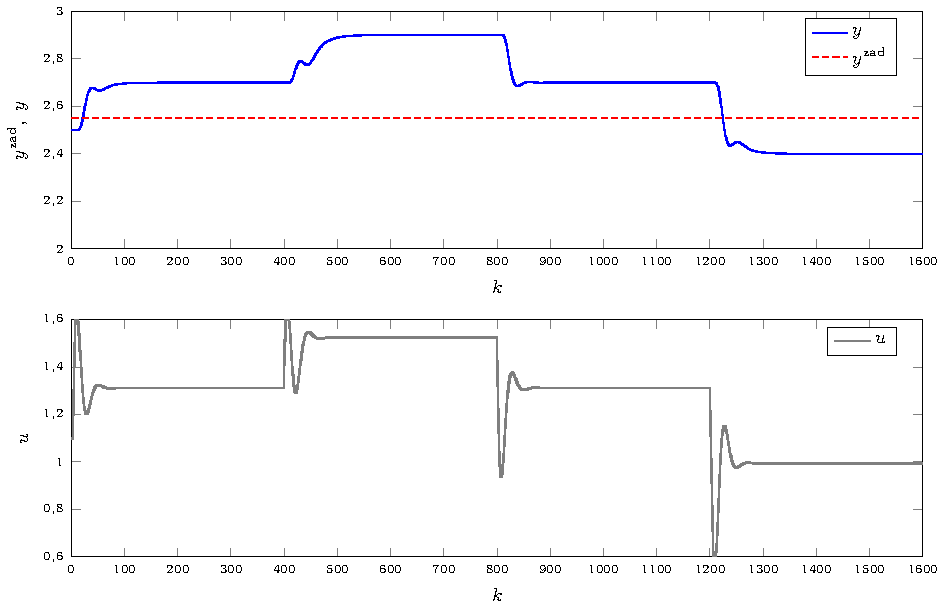
\includegraphics[scale=1]{rysunki/zapisz_pdf/DMC_D=200.000_N=27.00_Nu=27.00.pdf} 
\caption{Regulator DMC dla $D=200$, $N=27$, $N_{\mathrm{u}}=27$} 
\label{r_pgfplots_DMC_D=200.000_N=27.00_Nu=27.00} 
\end{figure}

\begin{figure}[tb] 
\centering 
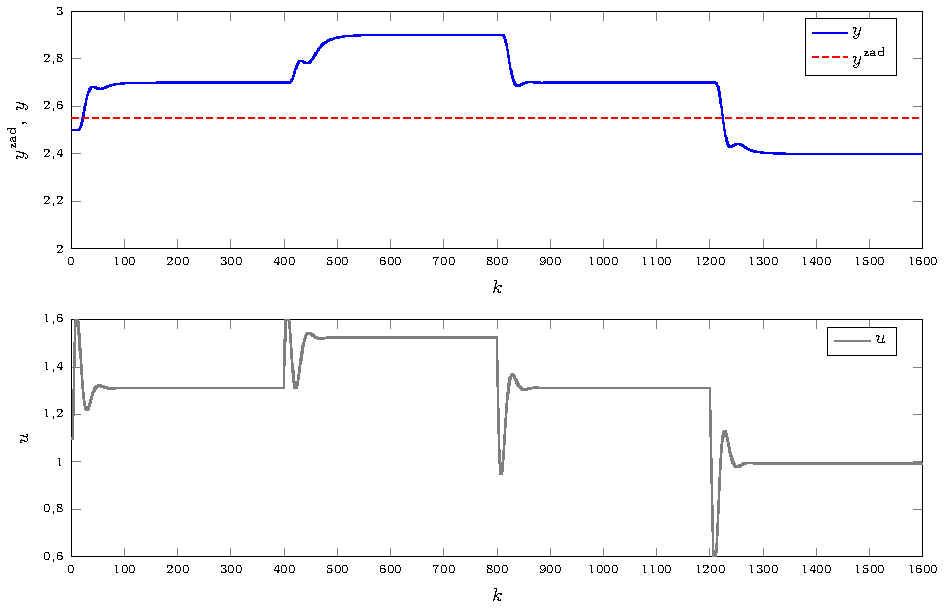
\includegraphics[scale=1]{rysunki/zapisz_pdf/DMC_D=200.000_N=32.00_Nu=32.00.pdf} 
\caption{Regulator DMC dla $D=200$, $N=32$, $N_{\mathrm{u}}=32$} 
\label{r_pgfplots_DMC_D=200.000_N=32.00_Nu=32.00} 
\end{figure}

\begin{table}
	[b] \caption{Porównanie wielkości błędu $E$ dla różnych wartości parametrów $N$ i $N_{\mathrm{u}}$ i dla parametru $D=200$}
	\label{t_T_i}
	\centering
	\sisetup{table-auto-round=true}
	\begin{small}
		\begin{tabular}{|c|c|}
			\hline
			$N$ i $N_{\mathrm{u}}$	&	$E$	\\
			$200$	&	$\num{4.8557}$		\\
			$150$ 	&	$\num{4.8557}$		\\
			$100$ 	&	$\num{4.8557}$ 		\\
			$50$ 	&	$\num{4.8556}$		\\
			$40$	&	$\num{4.8571}$	\\
			$35$	&	$\num{4.8403}$	\\
			$30$	&	$\num{4.8356}$	\\
			$32$	&	$\num{4.8301}$	\\
			$27$	&	$\num{4.8876}$	\\
			$25$	&	$\num{4.9796}$	\\
			$20$	&	$\num{5.3776}$	\\
			\hline
			\end{tabular}
	\end{small}
\end{table}

Większość przebiegów zapewnia zadowalający kształt funkcji wyjściowej, dlatego wybierając najlepszą wartość parametru $N$ kierować będziemy się wartością wskaźnika jakości $E$, co sprawia, że najlepszą regulację otrzymujemy dla $N=N_{\mathrm{u}}=32$. Wartość parametru $N_{\mathrm{u}}$ dobierana więc będzie dla $D=200$ i $N=32$. Ponieważ dla wartości $N_{\mathrm{u}}\ge{18}$ regulator zachowywał się w przybliżeniu identycznie nie zamieszczone zostały wykresy dla nich.

\begin{figure}[tb] 
\centering 
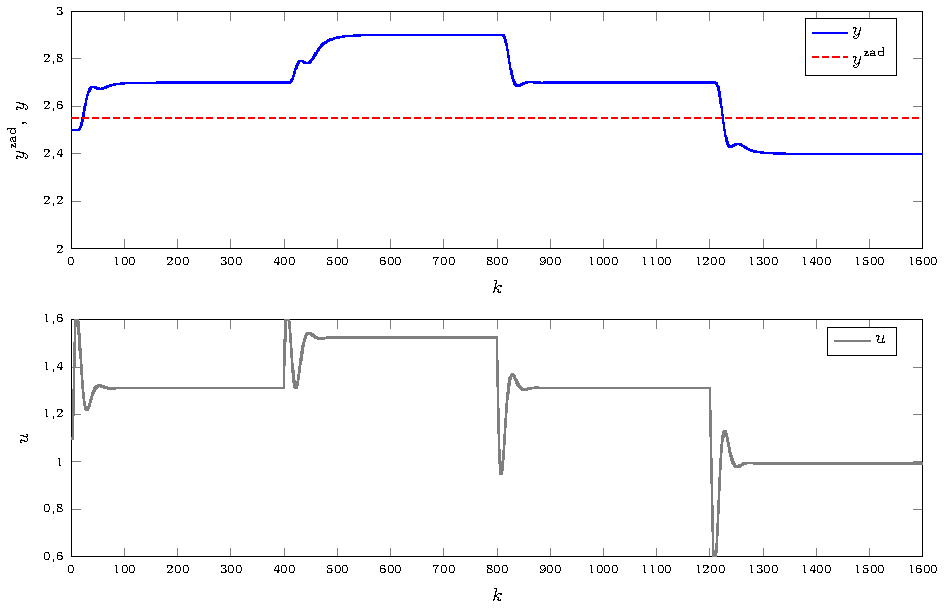
\includegraphics[scale=1]{rysunki/zapisz_pdf/DMC_D=200.000_N=32.00_Nu=15.00.pdf} 
\caption{Regulator DMC dla $D=200$, $N=32$, $N_{\mathrm{u}}=15$} 
\label{r_pgfplots_DMC_D=200.000_N=32.00_Nu=15.00} 
\end{figure}

\begin{figure}[tb] 
\centering 
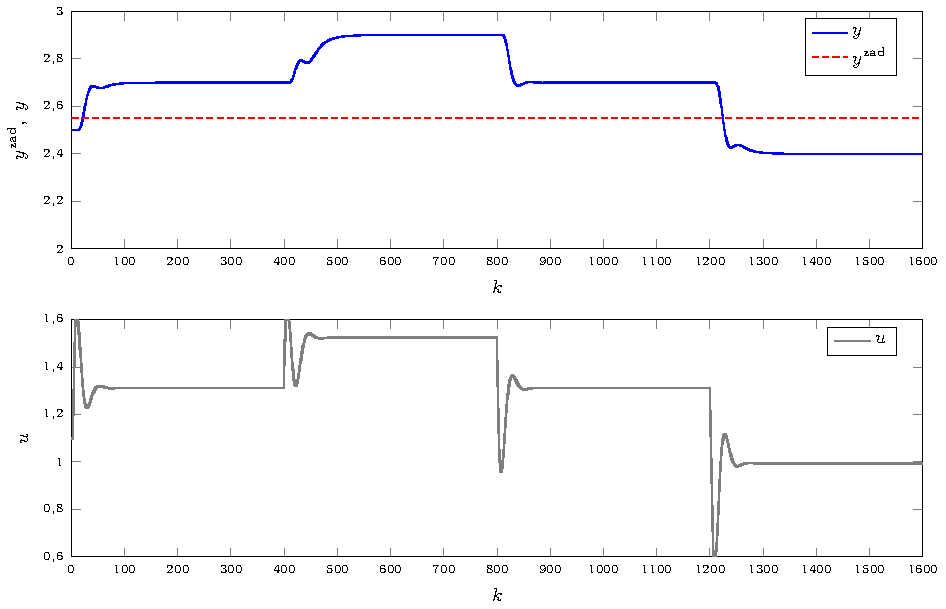
\includegraphics[scale=1]{rysunki/zapisz_pdf/DMC_D=200.000_N=32.00_Nu=10.00.pdf} 
\caption{Regulator DMC dla $D=200$, $N=32$, $N_{\mathrm{u}}=10$} 
\label{r_pgfplots_DMC_D=200.000_N=32.00_Nu=10.00} 
\end{figure}

\begin{figure}[tb] 
\centering 
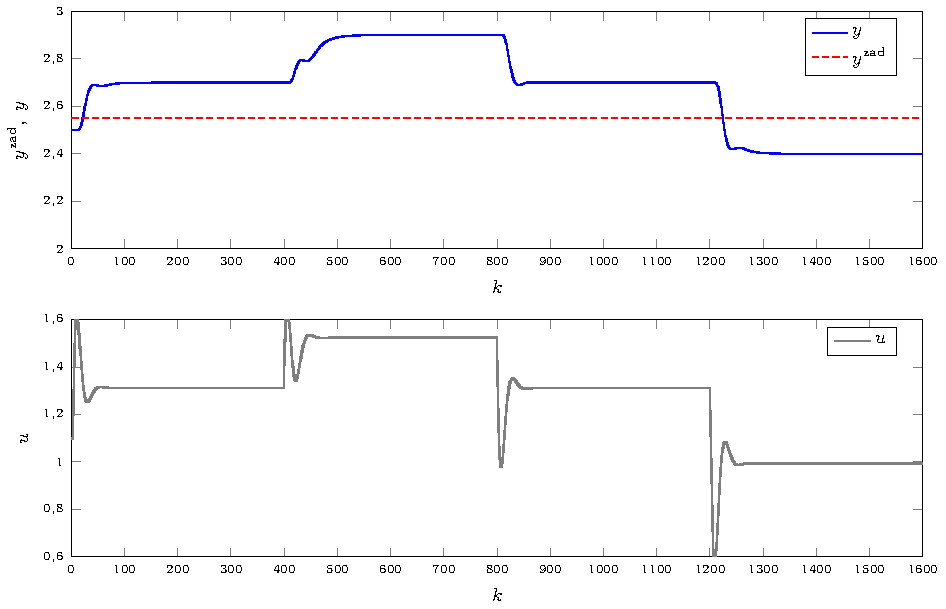
\includegraphics[scale=1]{rysunki/zapisz_pdf/DMC_D=200.000_N=32.00_Nu=7.00.pdf} 
\caption{Regulator DMC dla $D=200$, $N=32$, $N_{\mathrm{u}}=7$} 
\label{r_pgfplots_DMC_D=200.000_N=32.00_Nu=7.00} 
\end{figure}

\begin{figure}[tb] 
\centering 
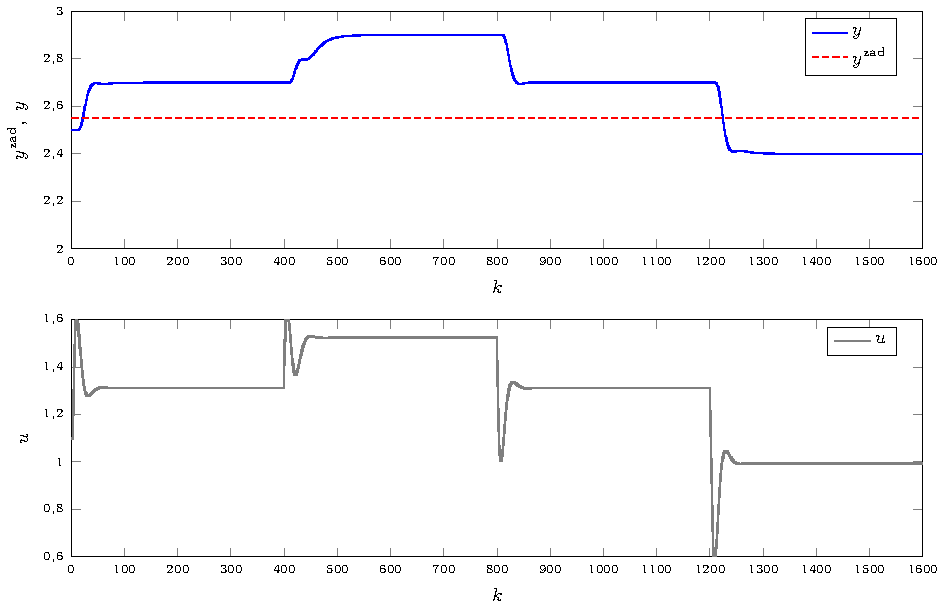
\includegraphics[scale=1]{rysunki/zapisz_pdf/DMC_D=200.000_N=32.00_Nu=5.00.pdf} 
\caption{Regulator DMC dla $D=200$, $N=32$, $N_{\mathrm{u}}=5$} 
\label{r_pgfplots_DMC_D=200.000_N=32.00_Nu=5.00} 
\end{figure}

\begin{figure}[tb] 
\centering 
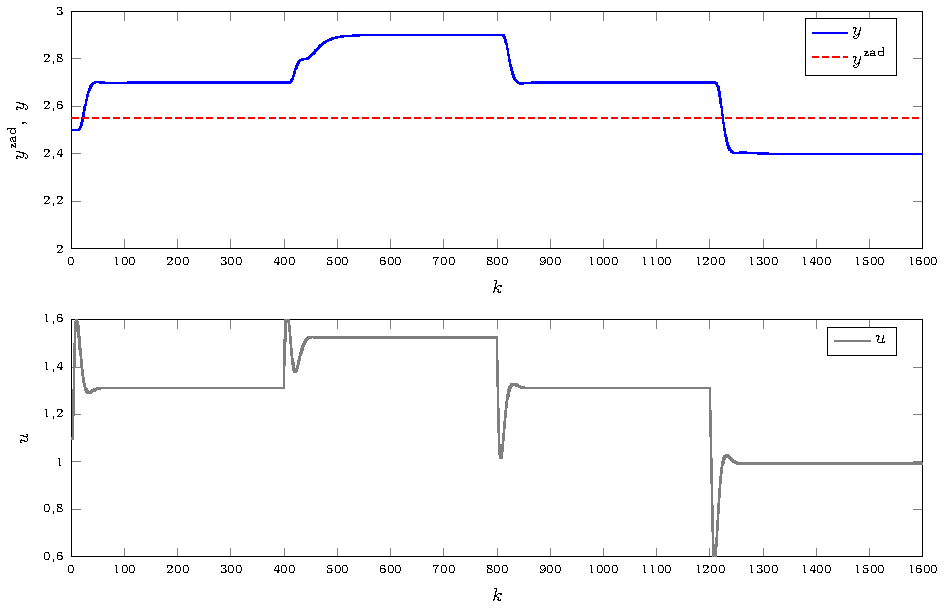
\includegraphics[scale=1]{rysunki/zapisz_pdf/DMC_D=200.000_N=32.00_Nu=4.00.pdf} 
\caption{Regulator DMC dla $D=200$, $N=32$, $N_{\mathrm{u}}=4$} 
\label{r_pgfplots_DMC_D=200.000_N=32.00_Nu=4.00} 
\end{figure}

\begin{figure}[tb] 
\centering 
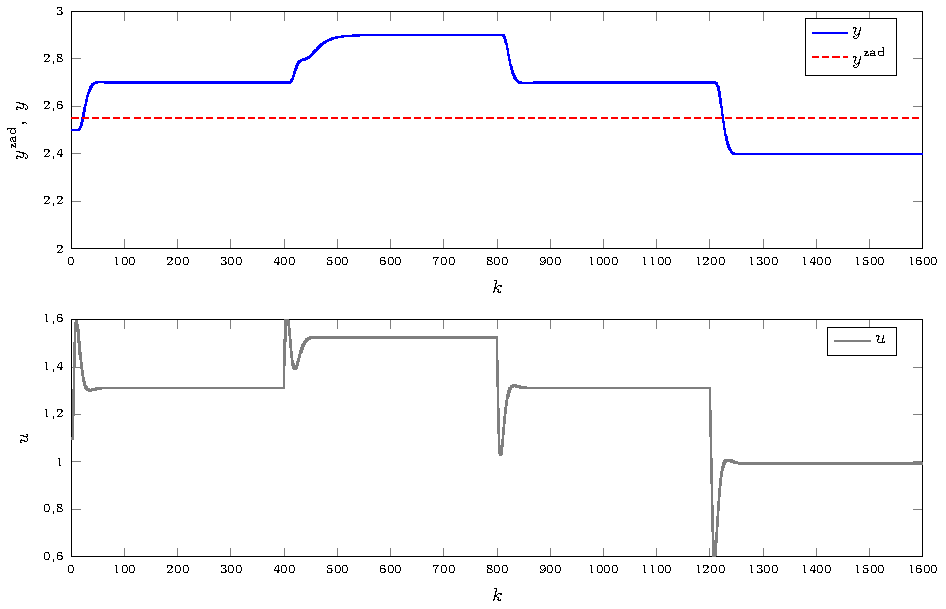
\includegraphics[scale=1]{rysunki/zapisz_pdf/DMC_D=200.000_N=32.00_Nu=3.00.pdf} 
\caption{Regulator DMC dla $D=200$, $N=32$, $N_{\mathrm{u}}=3$} 
\label{r_pgfplots_DMC_D=200.000_N=32.00_Nu=3.00} 
\end{figure}


\begin{table}
	[b] \caption{Porównanie wielkości błędu $E$ dla różnych wartości parametru $N_{\mathrm{u}}$ i dla parametrów $D=200$ i $N=32$}
	\label{t_T_i}
	\centering
	\sisetup{table-auto-round=true}
	\begin{small}
		\begin{tabular}{|c|c|}
			\hline
			$N_{\mathrm{u}}$	&	$E$	\\
			$32$	&	$\num{4.8301}$		\\
			$25$ 	&	$\num{4.8301}$		\\
			$20$ 	&	$\num{4.8301}$ 		\\
			$18$ 	&	$\num{4.8301}$		\\
			$15$	&	$\num{4.8288}$	\\
			$10$	&	$\num{4.8027}$	\\
			$7$		&	$\num{4.7471}$	\\
			$5$		&	$\num{4.7036}$	\\
			$4$		&	$\num{4.6905}$	\\
			$3$		&	$\num{4.7039}$	\\
			\hline
			\end{tabular}
	\end{small}
\end{table}


Dla różnych wartości parametru $N_{\mathrm{u}}$ przebiegi są w większości podobne, jedynie wartość wskaźnika jakości $E$ różni się nieznacznie między nimi. Z tego powodu, wybrany zostanie regulator o parametrach $D=200$, $N=32$ i $N_{\mathrm{u}}=4$ (Rys 6.31).

\chapter{Optymalizacja nastaw regulatora z użyciem dostępnych funkcji optymalizujących}
\section{Optymalizacja regulatora PID}


W  celu optymalizacji użyta zostanie funkcja \emph{fmincon} z Matlaba. Znajduje ona lokalne minimum funkcji na podstawie jej gradientu. Aby użyc jej do optymalizacji regulatora PID zdefiniowano funkcję ewaluującą jakość regulacji, która zwraca wskaźnik jakości $E$, a jako argument bierze wektor nastaw $K$, $T_{\mathrm{i}}$ i $T_{\mathrm{d}}$ regulatora. Funkcja \emph{fmincon} będzie starała się ten wskaźnik zminimalizować, zaczynając od podanego przez nas wektora nastaw. Funkcja ewaluująca zwraca wskaźnik jakości regulacji $E$. Wywołanie funkcji \emph{fmincon} wyglądać może na przykład tak:

\begin{lstlisting}
%wywolanie funkcji ewaluujacej regulator PID
x01 = [1.975, 24, 3];   %punkt poczatkowy optymalizacji
fmincon(@pid_eval, x01)   %wywolanie funkcji
\end{lstlisting}

Po znalezieniu przez funkcję \emph{fmincon} minimum lokalnego, możemy wprowadzić te parametry do skryptu z poprzedniego zadania, i sprawwdzić czy rzeczywiście działają lepiej. Na rysunku 7.1 przedstawiono odnalezione przez funkcję \emph{fmincon} rozwiazanie. Widać jednak, że otrzymany regulator pracuje w stanie ciągłych oscylacji, i mimo że są one bardzo małe (na tyle małe, że nie sprawiają dużej różnicy dla wskaźnika jakości $E$), są one niepożądane na obiektach realnych. Regulator ten średnio więc się nadaje do zastosowania na obiekcie realnym. Sposobem na poprawę, mogłoby być wprowadzenie jakiegoś dodatkowego współczynnika kary za oscylacje wokół wartości zadanej, bądź duże wydłużenie czasu w której wartość zadana jest stała, żeby spróbować skłonić \emph{fmincon} do faworyzowania nieoscylujących regulatorów. Rys 7.2 przedstawia regulator otrzymany w wyniku optymalizacji funkcją \emph{fmincon} dla ośmiokrotnie wydłużonej symulacji. Zgodnie z oczekiwaniami, otrzymany regulator PID ma dużo mniejsze tendencje do oscylowania. Dla bardziej wydłużonej symulacji, powinno móc się uzyskać regulator dużo mniej podatny na oscylacje. Przez to jednak, wskaźnik jakości jest nieco gorszy.


\begin{figure}[tb] 
\centering 
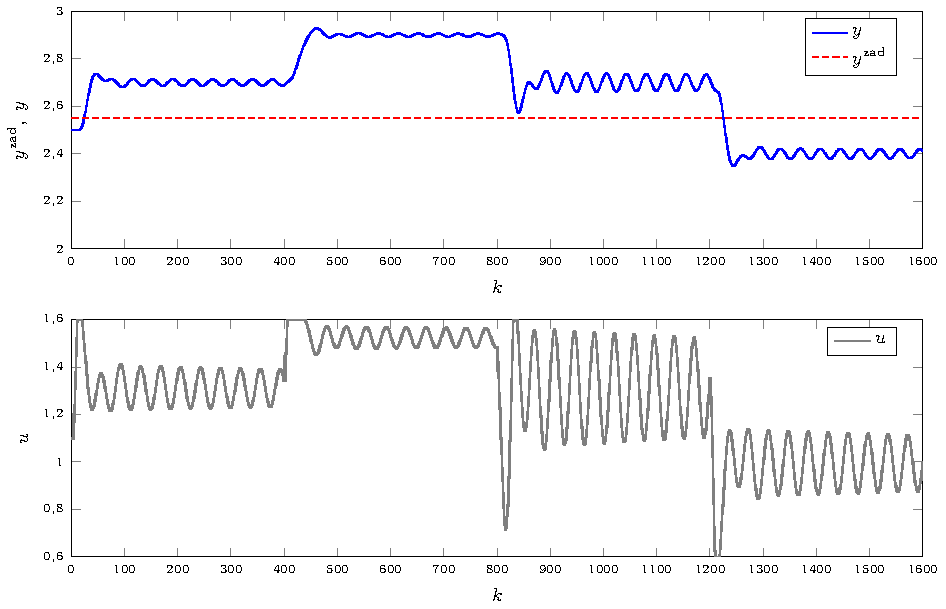
\includegraphics[scale=1]{rysunki/zapisz_pdf/PID_K=4.340_Ti=12.41_Td=8.10.pdf} 
\caption{Regulator PID $K=\num{4.34}$, $T_{\mathrm{i}}=\num{12.41}$, $T_{\mathrm{d}}=\num{8.1}$ otrzymany z punktu początkowego optymalizacji $K=\num{1.975}$, $T_{\mathrm{i}}=24$, $T_{\mathrm{d}}=3$} 
\label{r_pgfplots_PID_K=4.340_Ti=12.41_Td=8.10} 
\end{figure}

\begin{figure}[tb] 
\centering 
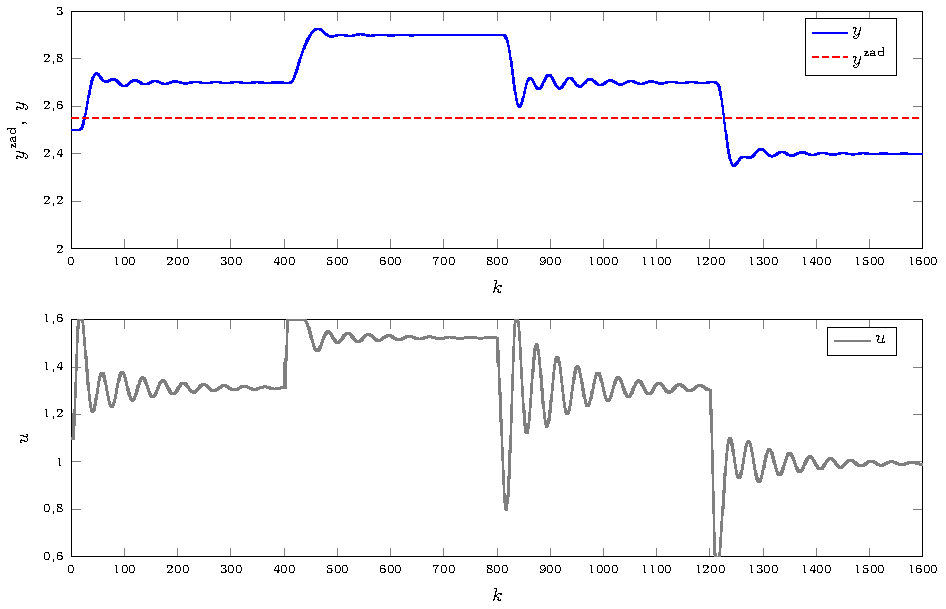
\includegraphics[scale=1]{rysunki/zapisz_pdf/PID_K=3.963_Ti=13.62_Td=7.87.pdf} 
\caption{Regulator PID $K=\num{3.963}$, $T_{\mathrm{i}}=13.62$, $T_{\mathrm{d}}=7.87$ otrzymany z punktu początkowego optymalizacji $K=\num{1.975}$, $T_{\mathrm{i}}=24$, $T_{\mathrm{d}}=3$} 

\label{r_pgfplots_PID_K=3.963_Ti=13.62_Td=7.87} 
\end{figure}




\begin{table}

	[b] \caption{Porównanie wielkości błędu $E$ dla różnych wartości parametru $T_{\mathrm{d}}$ i dla parametru $K=1.975$ oraz parametru $T_{\mathrm{i}}=24$}

	\label{t_T_i}
	\centering
	\sisetup{table-auto-round=true}
	\begin{small}
		\begin{tabular}{|c|c|c|c|}
			\hline
			$K$					&	$T_{\mathrm{i}}$	&	$T_{\mathrm{d}}$	&	$E$				\\
			$\num{4.3405}$		&	$\num{12.4148}$	&	$\num{8.097}$		&	$\num{5.0221}$	\\
			$\num{3.9628}$		&	$\num{13.6246}$	&	$\num{7.8695}$		&	$\num{5.1382}$	\\
			\hline
			\end{tabular}
	\end{small}
\end{table}

\section{Optymalizacja regulatora DMC}


W przypadku regulatora DMC niemożliwa jest optymalizacja funkcją \emph{fmincon}, ponieważ parametry regulatora DMC są zawsze dodatnimi liczbami całkowitymi. Z powodu użycia \emph{floor} w funkcji ewaluującej regulator DMC (analogiczna do funkcji ewaluującej regulator PID), funkcja \emph{fmincon} od razu zakończy optymalizację, twierdząc, że znalazła lokalne minimum. Jeżeli ma być odnaleziony najlepszy regulator DMC, należy użyć innej metody optymalizacji. Wybrana została funkcja \emph{ga} (,,Genetic Algorithm"), która jest częścią \emph{Global Optimization Toolbox} Matlaba. Wywołanie funkcji \emph{ga} może wyglądać tak:

\begin{lstlisting}
%wywolanie funkcji ewaluujacej regulator PID
x01 = [1.975, 24, 3];   %punkt poczatkowy optymalizacji
fmincon(@pid_eval, x01)   %wywolanie funkcji
%wywolanie funkcji ewaluujacej regulator DMC
A = [-1, 1];      
b = 0;          %ograniczenie liniowe -N+Nu<=0, czyli Nu<=N
Aeq = [];
beq = [];
lb = [1, 1];
ub = [200, 200];%ograniczenia wartosci N i Nu 1<=N<=200 i 1<=Nu<=200
nonlcon = [];
IntCon = [1, 2];    %pierwszy i drugi argument musza byc calkowite
ga(@dmc_eval,2,A,b,Aeq,beq,lb,ub,nonlcon,IntCon)
\end{lstlisting}

Tym spsobem otrzymaliśmy optymalne parametry regulatora DMC dla wybranej przez nas trajektorii wartości zadanej: $D=200$, $N=44$, $N_{\mathrm{u}}=5$. Regulator przedstawiony jest na Rys 7.3, a jego wskaźnik jakości $E=\num{4.6546}$. 

\begin{figure}[tb] 
\centering 
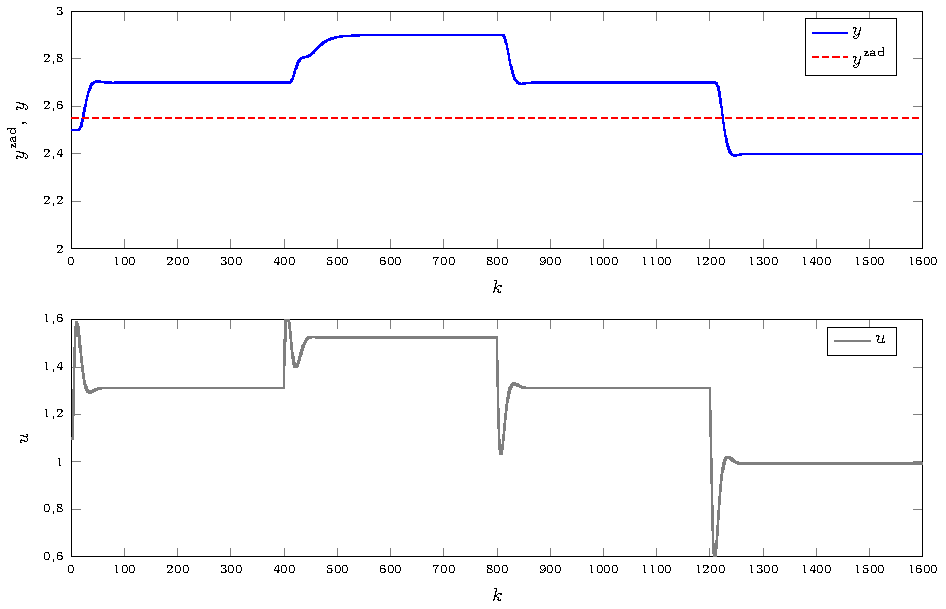
\includegraphics[scale=1]{rysunki/zapisz_pdf/DMC_D=200.000_N=44.00_Nu=5.00.pdf} 
\caption{Regulator DMC dla $D=200$, $N=44$, $N_{\mathrm{u}}=5$} 
\label{r_pgfplots_DMC_D=200.000_N=44.00_Nu=5.00} 
\end{figure}
\appendix
\end{document}

